\documentclass{llncs}
\bibliographystyle{splncs}
\renewcommand{\contentsname}{índice general}
\renewcommand\refname{Bibliografía}
\renewcommand\abstractname{Resumen}
\usepackage{listings}
\usepackage{indentfirst, enumitem,amsmath}
\usepackage[utf8]{inputenc}
\usepackage[spanish]{babel}
\usepackage[usenames, dvipsnames]{color}
\usepackage{comment}
\usepackage{algorithm}
\usepackage[noend]{algpseudocode}
\usepackage{amsmath}
\usepackage{amssymb}
\usepackage{graphicx}
\usepackage{float}
\usepackage{mathtools}
\usepackage{minted}
\usepackage{longtable}
\usepackage[long]{optidef}
\usepackage{subcaption}
\usepackage{multirow}
\captionsetup{compatibility=false}
\captionsetup[table]{skip=10pt}

\setcounter{secnumdepth}{3}
\newfloat{algorithm}{t}{lop}

\makeatletter
\def\BState{\State\hskip-\ALG@thistlm}
\makeatother

\makeatletter
\renewcommand{\ALG@name}{Algoritmo}
\newenvironment{breakablealgorithm}
{% \begin{breakablealgorithm}
	\begin{center}
		\refstepcounter{algorithm}% New algorithm
		\hrule height.8pt depth0pt \kern2pt% \@fs@pre for \@fs@ruled
		\renewcommand{\caption}[2][\relax]{% Make a new \caption
			{\raggedright\textbf{\ALG@name~\thealgorithm} ##2\par}%
			\ifx\relax##1\relax % #1 is \relax
			\addcontentsline{loa}{algorithm}{\protect\numberline{\thealgorithm}##2}%
			\else % #1 is not \relax
			\addcontentsline{loa}{algorithm}{\protect\numberline{\thealgorithm}##1}%
			\fi
			\kern2pt\hrule\kern2pt
		}
	}{% \end{breakablealgorithm}
		\kern2pt\hrule\relax% \@fs@post for \@fs@ruled
	\end{center}
}
\makeatother

\DeclarePairedDelimiter\abs{\lvert}{\rvert}
\newcommand{\expnumber}[2]{{#1}\mathrm{e}{#2}}

% Titulo
\title{Selección de Componentes Discretos para un Filtro Activo Mediante
  \textit{Programación por Restricciones} y \textit{Optimización por Colonia de Hormigas}} 
\author{Leandro Demarco Vedelago}
\institute{
            \email{leandrodemarco@gmail.com}\\
            Universidad Nacional de Córdoba, Fa.M.A.F
          }
\setcounter{tocdepth}{3}
\pagenumbering{arabic}
\pagestyle{plain}

%\setlength{\textwidth}{14cm}
%\setlength{\textheight}{21cm}


\begin{document}
{\def\addcontentsline#1#2#3{}\maketitle
  \noindent
  \makebox[\linewidth]{\small 25 de Marzo de 2017}}
  
\begin{abstract}
  Esto es el resumen 
\end{abstract}
% Fin titulo

%Tabla de contenidos
\tableofcontents
\newpage
%Fin tabla de contenidos
  \section{\textbf{Introducción}}
    \label{sec:motivacion}
    El dise\~no electrónico actual incluye a los filtros activos en muchas aplicaciones,
    tales como acondicionamiento y manipulación de se\~nales en frecuencias de audio e
    intermedias (IF) así como tareas de procesamiento digital de se\~nales. En
    contraposición a los filtros digitales, los activos pueden obtener buen rendimiento
    con demandas de potencia significativamente menores.
    
    Las alternativas de implementación de filtros activos presentan muchas opciones.
    Entre éstas, las implementaciones RC (resistencia/capacitor), construidas a partir de
    amplificadores operacionales, resistencias y capacitores son una de las más utilizadas
    por los ingenieros.\cite{corr}
    
    Un aspecto que cobra relevante importancia es la selección de los componentes discretos
    ya que el cumplimiento de las especificaciones depende en gran medida de ellos. Con el
    objetivo de realizar un diseño confiable los valores de los componentes pasivos se
    seleccionan de entre las series industriales E12, E24, E48, E96 o E192. Cada una de estas
    series limita el valor que puede tomar cada componente.
    
    A fin de obtener un diseño que satisfaga las especificaciones,  una posibilidad consiste 
    en enumerar todas las posibles combinaciones de valores para las resistencias y 
    capacitores que conforman el filtro y encontrar aquella que mejor las cumple. Sin embargo,
    dada la amplitud del rango de valores que cada componente puede adoptar el tamaño del
    espacio de soluciones suele ser inmanejable para adoptar este enfoque, con
    lo cual es necesario utilizar métodos o heurísticas de búsqueda que reduzcan el tiempo
    necesario.
    
    En la sección \ref{sec:fundelect} definimos el filtro analizado
    junto a los fundamentos electrónicos que definen la bondad del mismo. Luego, en la
    sección \ref{sec:fundprog} introducimos la noción de \textit{Programación por Restricciones} 
    (del inglés \textit{Constraint Programming})
    y cómo se define en términos de este paradigma el problema en cuestión. En la sección
    \ref{sec:exhaustSearch} presentamos una serie de observaciones y manipulaciones matemáticas 
    del problema que permiten obtener una solución analítica y definir un algoritmo exhaustivo que se ejecuta
    en tiempos razonables. Finalmente, en la sección \ref{sec:acor} presentamos la metaheurística ACO
    -del inglés \textit{Ant Colony Optimization}- aplicada a este problema junto a una variante 
    del mismo llamada ACO\textsubscript{$\mathbb{R}$}.
    
  \section{\textbf{Fundamentos electrónicos}}
    \label{sec:fundelect}
    Tomaremos como caso de estudio el mismo filtro que se utiliza en \cite{lov:rom:per}. Dicho filtro
    es de tipo IGMFB (Infinite-Gain Multiple Feedback) pasabajo de segundo orden. Son filtros
    bicuadráticos que emplean múltiples lazos de retroalimentación y un amplificador operacional.
    Una descripción más detallada de este tipo de filtros puede encontrarse en \cite{dim} y \cite{rau:swa}. 
    En la figura \ref{fig:filter} se muestra el esquemático del filtro a analizar.
   
   \begin{figure}
   	\centering
   	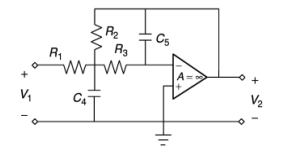
\includegraphics[scale=0.65]{filter.png}
   	\caption{Filtro IGMFB pasabajo de segundo orden.}
   	\label{fig:filter}
   \end{figure}

	Las especificaciones del filtro están dadas por la ganancia en la banda de paso ($G$), la
	frecuencia de polo ($\omega_p$) y el factor de calidad ($Q_p$). En función de estos valores
	la función de transferencia del filtro queda expresada de la siguiente manera:
 	\begin{equation}
		F(s) = \frac{G\omega_p^2}{s^2+(\frac{\omega_p}{Q_p})s+\omega_p^2}
		\label{funcTransfer}
	\end{equation}
	
	Para los filtros IGMFB los valores de $G$, $\omega_p$ y $Q_p$ pueden calcularse a partir
	de los valores de las resistencias y capacitores, de acuerdo a las siguientes fórmulas
	
	\begin{eqnarray}
		G &=& R_2/R_1 \label{defG} \\
		\omega_p &=& 1/\sqrt{R_2 R_3 C_4 C_5} \label{defOmega} \\
		Q^{-1}_p &=& \sqrt{C_5/C_4}  \left(\sqrt{R_2 R_3}/R_1 + \sqrt{R_3/R_2} +
		\sqrt{R_2/R_3}\right) \label{defQ}
	\end{eqnarray}
	
	\subsection{Sensibilidad de un filtro IGMFB}
	\label{subsec:sensFiltro}
	El término sensibilidad es utilizado para expresar una medida de
	la variación del rendimiento como resultado de cambios en los valores de los
	componentes. Dichas variaciones pueden ocurrir debido al envejecimiento de los
	mismos, tolerancias de fabricación, condiciones ambientales (temperatura), entre
	otros factores \cite{dim,rau:swa}. Mientras menos sensible es un filtro a los cambios en sus
	componentes, más estables permanecen sus características y, por lo tanto, existen más
	probabilidades de que pueda permanecer dentro de sus especificaciones,
	independientemente de la presencia de dichos cambios. Una ventaja de los filtros IGMFB es
	que presentan sensibilidades más bajas respecto a otros filtros bicuadráticos.
	
	De manera general, si $F$ es una función de varias variables, $F(x_1, x_2,...,x_n)$, entonces
	la sensibilidad de F con respecto a $x_i$ está definida por:
	\begin{equation}
		S_{x_i}^F = \frac{\%\ cambio\ en\ F}{\%\ cambio\ en\ x_i} = \frac{\partial F/F}{\partial x_i/x_i}
		\label{sensibilidad}
	\end{equation}
	
	Se considera que un filtro tiene baja sensibilidad cuando la sensibilidad respecto a cada uno
	de sus componentes es inferior a la unidad \cite{rau:swa}.
	
	Para el filtro de la figura (\ref{fig:filter}) las sensibilidades de $Q_p$ y $\omega_p$ con respecto a cada uno 
	de los componentes pasivos vienen dadas por las siguientes ecuaciones:
	
	\begin{eqnarray}
		S_{R_1}^{\omega_p} &=& 0 \label{sensR1Omega}\\
		S_{R_2}^{\omega_p} &=& S_{R_3}^{\omega_p} = S_{C_4}^{\omega_p} = S_{C_5}^{\omega_p} = -\left(\frac{1}{2}\right) \label{sensOtrosOmega}\\
		S_{C_4}^{Q_p} &=& - S_{C_5}^{Q_p} = \left(\frac{1}{2}\right) \label{sensCapQ}\\
		S_{R_1}^{Q_p} &=& Q_p \left(\frac{1}{R_1} \sqrt{\frac{R_2 R_3 C_5}{C4}}\right) \label{sensR1Q}\\
		S_{R_2}^{Q_p} &=& - \frac{Q_p}{2} \left(\frac{1}{R1} \sqrt{\frac{R_2 R_3 C_5}{C_4}} - \sqrt{\frac{R_3 C_5}{R_2 C_4}} + \sqrt{\frac{R_2 C_5}{R_3 C_4}}\right) \label{sensR2Q}\\
		S_{R_3}^{Q_p} &=& - \frac{Q_p}{2} \left(\frac{1}{R1} \sqrt{\frac{R_2 R_3 C_5}{C_4}} + \sqrt{\frac{R_3 C_5}{R_2 C_4}} - \sqrt{\frac{R_2 C_5}{R_3 C_4}}\right) \label{sensR3Q}
	\end{eqnarray}
	
	Las sensibilidades de las ecuaciones (\ref{sensR1Omega}), (\ref{sensOtrosOmega}) y (\ref{sensCapQ}) adoptan 
	valores fijos, mientras que las otras dependen de los valores que adopten los componentes. 
	En consecuencia, debemos considerar las sensibilidades (\ref{sensR1Q}), (\ref{sensR2Q}) y (\ref{sensR3Q}) 
	a la hora de seleccionar los valores para cada componente. 
	
	Idealmente, querríamos hallar una solución que minimice las tres sensibilidades $S_{R_1}^{Q_p}$, $S_{R_2}^{Q_p}$ y
	$S_{R_3}^{Q_p}$ simultáneamente. Dado que desconocemos si existe tal solución, definimos la \textit{sensibilidad total} del filtro:
	\begin{equation}
		S_T = S_{R_1}^{Q_p}  + S_{R_2}^{Q_p} + S_{R_3}^{Q_p}
	\end{equation} 
	e intentaremos minimizar dicha sensibilidad.
	
	En el caso de estudio seleccionado, la especificación elegida para el filtro es $G_{obj} = 3$,
	$\omega_{p_{obj}}=1000*2*\pi$ $rad/s$ y $Q_{p_{obj}} = 1 / \sqrt{2}$. 
	
	Consideraremos así mismo un escenario donde las resistencias y capacitores pueden tomar valores de la serie E24 y E12, con rangos en $10^3$-$10^6$$\Omega$ y $10^{-9}$-$10^{-6}$F, respectivamente. Se supone que valores fuera de estos rangos conducirían a efectos negativos debido a capacidades parásitas o señales de corriente muy grandes. De esta manera, el espacio de búsqueda total asciende a 
	$4.84*10^8$ alternativas. Se define además una tolerancia o error máximo $\epsilon_{max} = 2,5\%$ para los valores de $G_{obj}$,
	$\omega_{p_{obj}}$ y $Q_{p_{obj}}$.	
    
  \section{\textbf{Programación por Restricciones}}
    \label{sec:fundprog}
    Intuitivamente, los problemas de satisfacción de restricciones (\textit{CSP}, por sus siglas en inglés) pueden definirse como \textit{encontrar una solución que satisface determinadas restricciones o pro\-pie\-da\-des}. Muchos problemas de la vida real pueden ser reducidos a 
    este tipo de problemas, por ejemplo: el planeamiento y control del tráfico aéreo en un aeropuerto, el confeccionamiento de una agenda de clases o el diseño de una dieta saludable. 
    Todos estos problemas suelen ser \textit{NP}-Complejos.
    
   Existen dos técnicas para intentar solucionar este tipo de problemas \cite{sol}: una posibilidad es utilizar \textit{métodos exactos}, que exploran el espacio de combinaciones de forma exhaustiva estructurándolo como un árbol de búsqueda. Para acotar el problema de la
    explosión combinatoria, la búsqueda se combina con técnicas de filtrado, para
    \textit{podar} subconjuntos de combinaciones, y con heuristícas de ordenación, para orientar la búsqueda hacia las ramas más promisorias primero.
    
    Cuando las técnicas de filtrado y las heurísticas de ordenamiento no son suficientes para prevenir la explosión combinatoria, se debe dejar de lado la exhaustividad y utilizar \textit{métodos heurísticos} que exploran el espacio de búsqueda de forma incompleta, utilizando (meta)heurísticas para guiar la búsqueda hacia las áreas más promisorias ignorando deliberadamente otras áreas. Dentro de este enfoque hay dos variantes: las \textit{heurísticas perturbativas} -ej: Algoritmos Genéticos- que van modificando iterativamente combinaciones existentes a fin de crear nuevas combinaciones, y las \textit{heurísticas constructivas} que construyen nuevas combinaciones iterativamente desde cero.
    
    \subsection{Noción de una restricción}
      Una restricción puede pensarse como una relación lógica entre un conjunto de valores, en principio,
      desconocidos, también llamados \textit{variables}. De esta forma, una restricción restringe el conjunto
      de valores que pueden asignarse simultaneamente a sus variables.
      
      Una posibilidad para definirla consiste en enumerar todo el conjunto de tuplas que pertenece a la relación o,
      de manera dual, especificar aquellos que \textbf{no} pertenecen a ella.
      
      Existen diferentes tipos de restricciones, de acuerdo a los valores que pueden asignarse a las variables. Así,
      tenemos restricciones numéricas, booleanas, sobre conjuntos, etc. Una restricción numérica puede ser entonces
      una igualdad ($=$) o bien una desigualdad ($\neq, \geq, \leq, <, >$) entre dos expresiones aritméticas.
      
      De manera similar, las restricciones sobre conjuntos expresan relaciones entre variables cuyo rango son conjuntos y pueden
      incluir relaciones de igualdad ($=$), desigualdad ($\neq$), inclusión ($\subset, \subseteq$) o pertenencia ($\in$).
      
      Las restricciones sobre booleanos, pueden expresarse en términos de los operadores
      lógicos como por ejemplo $\wedge$, $\lor$, $\neg$, $\rightarrow$, etc.
      
    \subsection{Definición formal de un CSP}
    \label{subsec:cspformal}
      Se puede dar una definición formal de un CSP como sigue:
      
      Un CSP es una 3-upla (\textit{X}, \textit{D}, \textit{C}) tal que:
      \begin{itemize}
        \item \textit{X} es un conjunto finito de variables que corresponde a las incógnitas del problema.
        \item \textit{D} es una función que asocia un dominio \textit{D}($x_i$) con cada variable $x_i \in \textit{X}$, es
        decir \textit{D}($x_i$) es el conjunto de valores que la variable $x_i$ puede tomar.
        \item \textit{C} es un conjunto finito de restricciones y cada restricción $c_j \in C$ es una relación entre
        algunas variables de \textit{X}; este conjunto de variables se denota como $var(c_j).$
      \end{itemize}
  
  	Resolver un CSP $(X, D, C)$ consiste en asignar valores a todas las variables de forma tal
  	que todas las restricciones sean satisfechas. Más formalmente, se definen:
  	
  	- Una \textit{asignación} es un conjunto de pares (variables, valor) denotado
  	\begin{center}
  		{$A = \{(x_1, v_1), ..., (x_n, v_n)\}$} 
  	\end{center}
  	donde la misma variable no puede asignarse a dos valores distintos, es decir:
  	\begin{center}
  		{$\forall((x_i, v_i), (x_j,v_j)) \in A \times A,\ x_i = x_j \implies v_i = v_j$}
  	\end{center}
  	y el valor asignado a una variable pertenece a su dominio:
  	\begin{center}
  		{$\forall(x_i, v_i) \in A,\ v_i \in D(x_i)$}
  	\end{center}
     Se denota al conjunto de variables que tienen un valor asignado en la asignación $A$ como
     $var(A)$:
     \begin{center}
     	$var(A) = \{x_i \mid (x_i, v_i) \in A\}$
     \end{center}
 
   - Una asignación $A$ se dice \textit{completa} si asigna un valor a todas las variables del
   problema, es decir, si $var(A) = X$; en caso contrario se dice que es \textit{parcial}.
   
   - Una asignación $A$ \textit{satisface} una restricción $c_k$ tal que $var(c_k) \subseteq var(A)$ si la relación definida por $c_k$ es verdadera para los valores de las variables de $c_k$ definidos en $A$. Caso contrario, la asignación \textit{viola} la restricción.
   
   - Una asignación $A$ (completa o parcial) es \textit{consistente} si satisface todas las restricciones y es \textit{inconsistente} si viola al menos una.
   
   - Una \textit{solución} es una asignación completa y consistente.
   
   \subsection{Complejidad de un CSP}
   \label{subsec:cspComplexity}
   	Dado que los dominios pueden ser intervalos numéricos continuos, no todos los CSP son
   	problemas combinatorios. La complejidad teórica de un CSP depende del dominio de las variables y del tipo de restricciones utilizadas.
   	
   	En algunos casos, el problema puede ser polinomial. Este es el caso, por ejemplo, cuando todas
   	las restricciones son (in)ecuaciones lineales y todos los dominios son intervalos numéricos
   	continuos.
   	
   	En otros casos, el problema puede ser indecidible. Por ejemplo, cuando las restricciones pueden ser cualquier fórmula matemática arbitraria y los dominos de las variables son intervalos numéricos continuos.
   	
   	Sin embargo, en muchos casos, el problema es $\mathcal{NP}$-completo. En particular, los CSP con dominios finitos suelen pertenecer a este grupo en general.
   	
   	\subsection{Problemas de optimización relacionados a CSP}
   	\label{subsec:cspOptimization}
   	Los problemas de satisfacción de restricciones implican encontrar una solución que las
   	satisfaga a todas o bien probar la inconsistencia si no existe ninguna solución. Sin embargo,
   	en muchos casos también suelen haber involucrados problemas de optimización. En particular,
   	el resolver problemas \textit{excesivamente restringidos} suele convertirse en maximizar la
   	satisfacción de restricciones. Otras veces el resolver un CSP tambien involucra optimizar
   	alguna función objetivo al tiempo que se satisfacen todas las restricciones.
   	
   	\subsubsection{Maximización de satisfacción de restricciones}
   	Cuando las restricciones de un CSP son tales que no pueden ser todas satisfechas simultáneamente, se dice que el CSP está \text{excesivamente restringido}. En este caso,
   	usualmente se intenta hallar una asignación completa que satisfaga tantas restricciones como sea posible o, a la inversa, viole la menor cantidad posible. Este problema se llama \textit{CSP parcial} o \textit{MaxCSP} \cite{fre:wal}.

	También suele ocurrir en muchos problemas que no todas las restricciones sean igualmente
	importantes. Algunas pueden ser \textit{duras}, con lo cual no deben ser violadas, mientras
	que otras pueden ser \textit{blandas}, permitiendo que se las viole a algún costo dado. En este caso se le asocia un peso a cada restricción blanda que define el costo de violarla, y el objetivo es encontrar la asignación completa que satisface todas las restricciones duras y minimiza la suma ponderada de las restricciones blandas violadas. Este problema se llama CSP ponderado, (WCSP, por sus siglas en inglés) \cite{shi:far:ver}.
	
	Para estos CSP excesivamente restringidos, el espacio de búsqueda está definido por el
	conjunto de todas las asignaciones completas posibles y el objetivo es encontrar aquella que maximiza el nivel de satisfacción: el número de restricciones satisfechas en el caso de MaxCSP y
	la suma ponderada de las restricciones satisfechas en el caso los WCSP. En la mayoría de los
	casos, estos problemas son $\mathcal{NP}$-complejos ya que los problemas de decisión asociados son $\mathcal{NP}$-completos. Debe notarse además que son generalizaciones de
	CSP, con lo cual un algoritmo diseñado para resolver cualquiera de estos problemas puede
	utilizarse para resolver un CSP.
	
	\subsubsection{Optimización restringida}
	Cuando las restricciones de un CSP son tales que existen múltiples soluciones que las satisfacen a todas, el CSP se dice estar \textit{sub-restringido}. En este caso, algunas soluciones
	pueden ser preferibles a otras. Estas preferencias pueden ser expresadas añadiendo una función
	objetivo a ser maximizada (o minimizada), definiendo así un un problema de optimización
	restringida. Formalmente, un problema de optimización restringida está definido por un CSP
	$(X, D, C)$ y una función objetivo $f: X \rightarrow \mathbb{R}$. El objetivo es hallar una solución del CSP 
	que maximiza (o minimiza) $f$. En estos casos la dificultad no radica en hallar una solución, 
	si no en hallar una óptima con respecto a $f$.
	
	\subsection{Definición del problema del filtro como CSP}
		\label{subsec:problemDefinition}
		Como se estableció en la sección \ref{sec:fundelect}, el problema consiste en seleccionar
		los valores para las resistencias $R_1$, $R_2$ y $R_3$ y los capacitores $C_4$ y $C_5$ de
		una lista de posibles valores (las series industriales E12). Si definimos
		
		\begin{align*}
		G^{max} = G_F * (1 + \epsilon_{max})\\
		G^{min} = G_F * (1 - \epsilon_{max})\\
		\omega_p^{max} = \omega_{p_F} * (1 + \epsilon_{max})\\
		\omega_p^{min} = \omega_{p_F} * (1 - \epsilon_{max})\\
		Q_p^{max} = Q_{p_F} * (1 + \epsilon_{max})\\
		Q_p^{min} = Q_{p_F} * (1 - \epsilon_{max})
		\end{align*}
		
		Entonces el problema puede modelarse como un CSP $(X, D, C)$ donde:
		
		\begin{itemize}
			\item $X = \{R_1, R_2, R_3, C_4, C_5\}$
			\item $D(R_i) = E24, i \in \{1,2,3\}$ y $D(C_i) = E12, i \in \{4,5\}$
			\item $C = \{G^{max} > G_F > G^{min}, \omega_p^{max} > \omega_{p_F} > \omega_p^{min},
			Q^{max} > Q_F > Q^{min}\}$
		\end{itemize}
	
		Además, el problema está \textit{sub-restringido} dado que hay múltiples soluciones que satisfacen las restricciones.
		En nuestro caso, la preferencia entre las soluciones está determinada por aquella que presente menor sensibilidad total. 
		Es decir, $f: X \rightarrow \mathbb{R} = S_T(R_1, R_2, R_3, C_4, C_5)$ y queremos minimizarla.
		
		Como mencionamos en la sección \ref{subsec:sensFiltro}, idealmente querríamos hallar una solución que minimice las tres
		sensibilidades simultáneamente, pero desconocemos si existe o no tal solución, por lo cual hemos definido la sensibilidad total
		$S_T$ como la suma de cada una de las tres sensibilidades. Otra posibilidad consistiría en ver, dado un conjunto
		de soluciones, cuáles de ellas son \textit{óptimos de Pareto} de acuerdo a las siguientes definiciones:
		\begin{itemize}
			\item Dados dos vectores $\vec{u} = (u_1, \dots, u_k)$ y $\vec{v} = (v_1, \dots, v_k)$, se dice que $\vec{u}$ \textit{domina}
			a $\vec{v}$ si y sólo si $\bigl<\forall i : i \in {1, \dots, k} : u_i \leq v_i\bigr>$.
			\item Dado un conjunto de vectores $S$, se dice que $\vec{v}^{\star} \in S$ es un \textit{óptimo de Pareto} si y sólo si
			$\neg \bigl<\exists \vec{v'} : \vec{v'} \in S \wedge \vec{v'} \neq \vec{v} : \vec{v'} \text{ domina a } \vec{v}\bigr>$.
		\end{itemize}
	
	  En nuestro caso, dadas dos soluciones:
	  \begin{align*}
	  		S^1 = (R_1^1, R_2^1, R_3^1, C_4^1, C_5^1)\\
	  		S^2 = (R_1^2, R_2^2, R_3^2, C_4^2, C_5^2)\\
	  \end{align*}
	  diremos que $S^1$ domina a $S^2$ si y sólo si $S_{R_1}^{Q_p}(S^1) \leq S_{R_1}^{Q_p}(S^2) \wedge S_{R_2}^{Q_p}(S^1) \leq S_{R_2}^{Q_p}(S^2) \wedge S_{R_3}^{Q_p}(S^1) \leq S_{R_3}^{Q_p}(S^2)$
	  
	\section{\textbf{Algoritmo Exhaustivo}}
		\label{sec:AlgoritmoExhaustivo}
		En esta sección mostraremos cómo realizando algunas observaciones y operaciones matemáticas 
		es posible obtener un algoritmo exhaustivo que encuentra todas las soluciones posibles para el problema.
		
		Es claro que a partir de (\ref{defG}) se tiene que para cada valor de $R_1$ hay un conjunto de valores 
		de $R_2$ que denotaremos  $\{R_2\}_{R_1}$ tales que $G^{max} > G > G^{min}$
		
		Definiendo las siguientes frecuencias,
		\begin{eqnarray}
		\omega_1 &=& 1/(R_2 C_4) \nonumber \\
		\omega_2 &=& 1/(R_3 C_5)
		\label{omegas}
		\end{eqnarray}
		podemos reescribir (\ref{defOmega}) de la siguiente forma: $\omega_p = \sqrt{\omega_1  \omega_2}$
		
		A partir de los valores que pueden tomar las resistencias y capacitores, es posible calcular la lista de 
		valores que pueden tomar las frecuencias definidas en (\ref{omegas}).
		
		Para cada uno de los valores posibles para $\omega_1$, habrá un conjunto de pares de valores ($R_2$, $C_4$) tales que
		$\omega_1 = 1/(R_2 C_4)$. Designamos a tal conjunto como $\{(R_2,C_4)\}_{\omega_1}$. 
		
		De manera análoga se puede proceder con $\omega_2$, $R_3$ y $C_5$ (obsérvese que el conjunto de valores 
		posibles para $\omega_2$ es el mismo que para $\omega_1$ y que $\{(R_2,C_4)\}_{\omega_1}=\{(R_3,C_5)\}_{\omega_2}$ 
		cuando $\omega_1=\omega_2$). 
		
		Luego, dada la restricción $\omega_p \in  [\omega_p^{min},\omega_p^{max}]$ y 
		elegido un valor de  $\omega_1$, los valores admisibles de $\omega_2$ son aquellos para los que 
		$\omega_p= \sqrt{\omega_1 \omega_2}$ satisface dicha restricción, y por lo tanto cumplen las siguiente relación:
		\begin{equation*}
		\frac{(\omega_p^{max})^2}{\omega_1} > \omega_2 > \frac{(\omega_p^{min})^2}{\omega_1}
		\end{equation*}
		
		De esta manera, para cada valor realizable de $\omega_1$ existe un conjunto finito $\{{\omega_2}\}_{\omega_1}$ 
		de valores de $\omega_2$ tales que $ \omega_p^{max} > \omega_p > \omega_p^{min} $
		
		Por otro lado, a partir de (\ref{defQ}) y (\ref{omegas}) podemos reescribir $Q_p^{-1}$ de la siguiente forma,
		\begin{equation}
		Q_p^{-1} =
		\sqrt{\frac{\omega_1}{\omega_2}}\left(1+\frac{R_2}{R_1}+\frac{R_2}{R_3}\right)
		\label{otraq}
		\end{equation}
		
		Finalmente, para cada par ($R_1$, $R_2$), ($\omega_1, \omega_2$) que satisface
		las restricciones sobre $G$ y $\omega_p$, utilizando la expresión
		(\ref{otraq}) buscamos los valores $R_3$ admisibles que satisfagan la  condición
		$$
		(Q_p^{-1})^{max} > Q_p^{-1} > (Q_p^{-1})^{min}
		$$
		y de esta manera obtenemos todas las soluciones de la forma ($R_1$, $R_2$,
		$\omega_1$, $\omega_2$, $R_3$)  
		que luego podemos \textit{mapear} a las soluciones de la forma ($R_1$,
		$R_2$, $R_3$, $C_4$, $C_5$). 
		
		A continuación mostramos el \textit{pseudocódigo} del algoritmo de búsqueda exhaustiva que acabamos
		de describir.
		
		\begin{algorithm}[H]
			\caption{Búsqueda exhaustiva}
			\label{alg:exhaustSearch}
			\begin{algorithmic}[1]
				\State $R_{vals}$: conjunto de valores que pueden tomar las resistencias
				\State $C_{vals}$: conjunto de valores que pueden tomar los capacitores
				\State $G^{min}$: valor mínimo aceptable para la ganancia
				\State $G^{max}$: valor máximo aceptable para la ganancia
				\State $\omega_p^{min}$: valor mínimo aceptable para la frecuencia de polo
				\State $\omega_p^{max}$: valor máximo aceptable para la frecuencia de polo
				\State $Q^{min}$: valor mínimo aceptable para el factor de calidad
				\State $Q^{max}$: valor máximo aceptable para el factor de calidad
				\item[]
				\Procedure{ExhaustiveSearch}{$R_{vals}$, $C_{vals}$}
				\State $soluciones \gets []$
				\State $G_{constraint} \gets  []$ \Comment{Obtener pares $(r1,r2)$ que satisfagan la restricción sobre G}
				\For{cada $r1$ en $R_{vals}$, cada $r2$ en $C_{vals}$}
				\State $G \gets r2/r1$
				\If{$G^{max} > G > G^{min}$}
				\State Agregar el par $(r1, r2)$ a $G_{constraint}$
				\EndIf 
				\EndFor
				\item[]
				\State $\omega_{constraint} \gets \{\}$ \Comment{Diccionario que para cada $\omega_1$ contiene el conjunto de los $\omega_2$ posibles para no violar la
					restricción}
				\State $wToRCMap \gets \{\}$  \Comment{Diccionario que para cada valor de $w$ contiene una lista con los pares $(r,c)$ que lo generan}
				\item[]
				\State $w_{vals} = [ ]$
				\For{cada $r$ en $R_{vals}$, cada $c$ en $C_{vals}$}
				\State $w \gets 1/(r*c)$
				\State Agregar el par $(r,c)$ a $wToRCMap[w]$
				\State Agregar $w$ a la lista $w_{vals}$
				\EndFor
				\For{cada $w_1$ en $w_{vals}$}
				\State $Posibles\_\omega_2 \gets [ ]$
				\For{cada $w_2$ en $w_{vals}$}
				\State $minVal \gets {(\omega_p^{min})}^{2}$
				\State $maxVal \gets {(\omega_p^{max})}^{2}$
				\If{$maxVal > w2 > minVal$}
				\State Agregar $w2$ a la lista $Posibles\_\omega_2$
				\EndIf
				\EndFor
				\If{$Posibles\_\omega_2$ no es vacía}
				\State Agregar $Posibles\_\omega_2$ a $\omega_{constraint}[\omega_1]$
				\EndIf
				\EndFor
				\item[]
				\For{cada par $(r1,r2)$ en $G_{constraint}$}
				\For{cada $\omega_1$ en las keys de $\omega_{constraint}$}
				\State $Posibles\_\omega_2 \gets \omega_{constraint}[\omega_1]$
				\State $genera \gets \exists (r,c) \in wToRCMap[\omega_1] \mid r = r_2$ \Comment{Chequear si $r_2$ \textit{genera} $\omega_1$}
				\If{$genera$}
				\For{cada $\omega_2$ en $Posibles\_\omega_2$, cada $r_3$ en $R_{vals}$}
				\State $genera \gets \exists (r,c) \in wToRCMap[\omega_2] \mid r = r_3$ \Comment{Chequear si $r_3$ \textit{genera} $\omega_2$}
				\If{$genera$}
				\State $(Q^{-1})_{r_3} \gets \sqrt{\omega_1 / \omega_2} * (1  + r_2/r_1 + r_2/r_3)$
				\If{$(Q^{min})^{-1} > (Q^{-1})_{r_3} > (Q^{max})^{-1}$}
				\State $c_4 \gets 1/(r_2 * \omega_1)$
				\State $c_5 \gets 1/(r_3 * \omega_2)$ 
				\State Agregar la tupla $(r_1, r_2, r3, c4, c5)$ a la lista $soluciones$
				\EndIf
				\EndIf
				\EndFor
				\EndIf
				\EndFor
				\EndFor
				\State \textbf{return} $soluciones$
				\EndProcedure
			\end{algorithmic}
		\end{algorithm}
		
		El código \textit{Python} para este algoritmo puede encontrarse en el apéndice \ref{subsec:pythonexhaustivo}.

  \section{\textbf{Solución Analítica}}
    En esta sección presentaremos una solución analítica del problema que permite encontrar todas las soluciones del problema. 
    La ventaja de contar con una solución de este tipo es que nos permitirá evaluar luego el rendimiento de los métodos heurísticos, 
    en este caso en particular de ACO\textsubscript{$\mathbb{R}$}.
  	\label{sec:solAnalitica}
	  	El problema consiste en minimizar una función -la sensibilidad- de cinco variables -las tres resistencias y los dos capacitores-, 
	  	sujeta a tres restricciones,
	  	
	  	\begin{mini}
	  		{R_i,C_j}{S(R_i,C_j)}{}{}
	  		\addConstraint{G(R_i,C_j)}{\in [G_-,G_+]}{}
	  		\addConstraint{\omega(R_i,C_j)}{\in [\omega_-,\omega_+]}{}
	  		\addConstraint{Q(R_i,C_j)}{\in [Q_-,Q_+]}{}
	  		\label{opti}
	  	\end{mini}
  	    con $i=1,\ldots,3$ y $j=4,5$ y siendo
  	  	\begin{eqnarray}
	  	   G(R_i,C_j)&=&R_2/R_1 \label{g}\\
	  	   \omega(R_i,C_j)&=&\frac{1}{\sqrt{R_2C_4R_3C_5}}\label{omega}\\
	  	   Q(R_i,C_j)&=&\sqrt{\frac{C_4}{C_5}}\left\{\frac{\sqrt{R_2R_3}}{R_1} +
	  	   \sqrt{\frac{R_3}{R_2}} +\sqrt{\frac{R_2}{R_3}}\right\}^{-1} \label{q}\\
	  	   S(R_i,C_j)&=& \frac{1}{2} Q \sqrt{\frac{C_5}{C_4}} \left\{ 2 \left|
	  	   \frac{\sqrt{R_2R_3}}{R_1} \right| + \left| \frac{\sqrt{R_2R_3}}{R_1} -
	  	   \sqrt{\frac{R_3}{R_2}} +\sqrt{\frac{R_2}{R_3}} \right| + \right. \nonumber\\
	  	   && \left. \left| \frac{\sqrt{R_2R_3}}{R_1} +
	  	   \sqrt{\frac{R_3}{R_2}} - \sqrt{\frac{R_2}{R_3}} \right|\right\}\label{sens}
  	   \end{eqnarray}
  	   
  	   En el problema (\ref{opti}) los intervalos están todos especificados en base al
  	   error admisible respecto a un valor objetivo. Suponiendo el mismo error
  	   $\epsilon$ para todas las variables, y siendo los valores objetivos $G_0$,
  	   $\omega_0$ y $Q_0$ resulta
  	   \begin{eqnarray}
  	   G_\pm&=&(1\pm\epsilon)G_0\\
  	   \omega_\pm&=&(1\pm\epsilon)\omega_0\\
  	   Q_\pm&=&(1\pm\epsilon)Q_0
  	   \end{eqnarray}
  	   Para simplificar la discusión por ahora consideremos el problema (\ref{opti})
  	   ahora con variables continuas en lugar de discretas lo que permite considerar el
  	   problema de optimización con restricciones de igualdad (si no considerásemos
  	   variables continuas, el problema con restricciones de igualdad no tendría
  	   solución),  
  	   \begin{mini}
	  	   	{R_i,C_j}{S(R_i,C_j)}{}{}
	  	   	\addConstraint{G(R_i,C_j)}{= G_0}{}
	  	   	\addConstraint{\omega(R_i,C_j)}{=\omega_0}{}
	  	   	\addConstraint{Q(R_i,C_j)}{=Q_0}{}
	  	   	\label{opti2}
  	   \end{mini}
     
	A partir de (\ref{q}) y (\ref{sens}) es fácil ver que la sensibilidad depende sólo de los valores de las resistencias,
	\begin{eqnarray}
	S(R_1,R_2,R_3)&=&\frac{1}{2} \left\{\frac{\sqrt{R_2R_3}}{R_1} +
	\sqrt{\frac{R_3}{R_2}} +\sqrt{\frac{R_2}{R_3}}\right\}^{-1} \times 
	\left\{ 2 \left| \frac{\sqrt{R_2R_3}}{R_1} \right| + \right. \nonumber \\
	&& \left. \left| \frac{\sqrt{R_2R_3}}{R_1} -
	\sqrt{\frac{R_3}{R_2}} +\sqrt{\frac{R_2}{R_3}} \right| + 
	\left| \frac{\sqrt{R_2R_3}}{R_1} +
	\sqrt{\frac{R_3}{R_2}} - \sqrt{\frac{R_2}{R_3}} \right|\right\} \label{sens2}
	\end{eqnarray}
	
	Pero de (\ref{sens2}) se puede ver que la sensibilidad depende de los cocientes
	entre pares de resistencias, por lo que siendo tres las resistencias, dependerá
	sólo de dos cocientes independientes. Tomemos tales cocientes los siguientes,
	\begin{eqnarray}
	a&=&R_1/R_2\nonumber\\
	b&=&R_1/R_3 \label{variables}
	\end{eqnarray}
	En funci\'on de estas dos nuevas variables, la sensibilidad toma la forma,
	\begin{equation}
	S(a,b)=\frac{1}{2}\frac{\left\{ 2+\left|1-a+b\right| + \left|1+a-b\right|
		\right\} }{(1+a+b)}
	\end{equation}
	Teniendo en cuenta que en funci\'on de las nuevas variables $a$ y $b$ la ganancia
	es simplemente $G(a)=1/a$, el problema (\ref{opti2}) queda reducido a,
	\begin{mini}
		{a,b}{S(a,b)}{}{}
		\addConstraint{a}{= a_0}{}
		\addConstraint{\omega(R_i,C_j)}{=\omega_0}{}
		\addConstraint{Q(R_i,C_j)}{=Q_0}{}
		\label{opti3}
	\end{mini}
	donde definimos $a_0=1/G_0$. Teniendo en cuenta entonces que la restricci\'on
	sobre la ganancia no hace m\'as que fijar el valor de $a$ en $a_0$, resulta
	entonces que la 
	sensibilidad es funci\'on s\'olo de $b$. La minimizaci\'on de $S$ es entonces un
	problema de una sola variable. Para simplificar la notaci\'on definamos $d=1+a$
	con lo que la sensibilidad queda,
	\begin{equation}
	S(b)=\frac{1}{2}\frac{\left\{ 2+\left|2-d+b\right| + \left|d-b\right|
		\right\} }{(d+b)}
	\label{sens3}
	\end{equation}
	
	La presencia de la función valor absoluto introduce dos puntos en la función $S(b)$ en los que su derivada es
	discontinua: $b=d-2$ y $b=d$. Entonces el o los mínimos de $S$ estarán en
	los puntos donde la derivada sea nula, en los puntos de discontinuidad de la
	derivada o en los extremos del dominio. Si suponemos que la ganancia es mayor
	que 1, entonces $a<1$ y por lo  tanto $d<2$ con lo que el punto de discontinuidad de la derivada 
	$b=d-2$ no es de interés ya que es negativo y $b$ sólo puede tomar valores positivos. Un
	cálculo explícito permite mostrar que no existe ningún punto en el que la derivada
	se anule (para valores positivos de $b$). Respecto a los extremos del dominio,  si bien la función está definida 
	para $b\in(-\infty,+\infty)$, los valores negativos de $b$ no son de interés. Consideramos entonces  la función 
	$S(b)$ definida en $(0,+\infty)$ (aunque estrictamente hablando, 0 y $+\infty$ tampoco son valores
	realizables). A partir de (\ref{sens3}) obtenemos $S(0)=2/d>1$, $\lim_{b\to +\infty}  S(b)=1$ y el valor de $S$ 
	en el punto $b_0=d=1+a_0$ de discontinuidad de la derivada $S(b_0)=1/d$. Por lo tanto
	\begin{equation}
	\text{min} \;S(b)=S(d)=1/d
	\end{equation}
	Siendo $S(0)$ el máximo de la función (en el intervalo $(0,+\infty)$).
	
	Resumiendo lo hecho hasta ahora, el problema se redujo al siguiente sistema de ecuaciones,
	\begin{eqnarray}
	a&=&a_0\label{a}\\
	b&=&1+a\label{b}\\
	\omega(R_2,R_3,C_4,C_5)&=&\omega_0\label{omega2}\\
	Q(R_1,R_2,R_3,C_4,C_5)&=&Q_0\label{q2}
	\label{opti4}
	\end{eqnarray}
	
	Hemos llegado entonces a un sistema de 4 ecuaciones con 5 incógnitas, por lo tanto una variable es
	libre. Como el valor de $a$ está fijo por la primer ecuación, la segunda ecuación permite obtener el valor de $b$. 
	Las últimas dos ecuaciones, estando ya determinados los valores de $a$ y $b$, y teniendo en cuenta a partir de
	(\ref{variables}) que $R_2$ y $R_3$ se pueden expresar en función de $R_1$, $a$ y $b$, es un sistema de dos ecuaciones 
	con tres  incógnitas ($R_1$, $C_4$ y $C_5$). Elegimos como variable libre a $R_1$. Entonces, asignando a $R_1$ un valor, 
	dentro del rango admisible, las últimas dos ecuaciones permiten determinar los valores de los capacitores.
	
	Fijando el valor de $R_1$, de (\ref{a}) obtenemos $R_2$ y con (\ref{b}) $R_3$. Luego, de (\ref{omega2}) y 
	(\ref{q2}) obtenemos $C_4$ y $C_5$. El resultado final es,
	\begin{eqnarray}
	\label{eqarr:solAnalitica}
	R_2&=&G_0 R_1\nonumber\\
	R_3&=&\frac{R_1 R_2}{R_1+ R_2}\nonumber\\
	C_4&=&\frac{Q_0 D}{\omega_0 E}\\
	C_5&=&\frac{D E}{\omega_0 Q_0}\nonumber\label{final}
	\end{eqnarray}
	donde hemos definido,
	\begin{eqnarray}
	D&=&1/\sqrt{R_2 R_3}\nonumber\\
	E&=&\left\{\frac{\sqrt{R_2R_3}}{R_1} +
	\sqrt{\frac{R_3}{R_2}} +\sqrt{\frac{R_2}{R_3}}\right\}^{-1}
	\end{eqnarray}
	
	A modo de ejemplo mostramos en el cuadro \ref{cuadro1} el resultado de utilizar (\ref{final}) con los valores de $R_1$ del escenario 2. 
	Luego de calcular el conjunto de valores $(R_1,R_2,R_3,C_4,C_5)$ para cada valor de $R_1$, descartamos todas la
	tuplas en las que alguno de sus cinco elementos se salen del rango correspondiente al escenario.
	
	\begin{table}[!h]
          \begin{minipage}{0.5\textwidth}
		$$
		\begin{array}{|c|c|c|c|c|}
		\hline
		R_1    & R_2  & R_3   & C_4                          & C_5 \\
		\hline
		1500. & 4500. & 1125. & 2.00*10^{-7} & 2.50*10^{-8} \\
		1600. & 4800. & 1200. & 1.87*10^{-7} & 2.34*10^{-8} \\
		1800. & 5400. & 1350. & 1.66*10^{-7} & 2.08*10^{-8} \\
		2000. & 6000. & 1500. & 1.50*10^{-7} & 1.87*10^{-8} \\
		2200. & 6600. & 1650. & 1.36*10^{-7} & 1.70*10^{-8} \\
		2400. & 7200. & 1800.     & 1.25*10^{-7} & 1.56*10^{-8} \\
		2700. & 8100. & 2025.     & 1.11*10^{-7} & 1.38*10^{-8} \\
		3000. & 9000. & 2250.     & 1.00*10^{-7} & 1.25*10^{-8} \\
		3300. & 9900. & 2475.     & 9.09*10^{-8} & 1.13*10^{-8} \\
		3600. & 10800. & 2700.    & 8.33*10^{-8} & 1.04*10^{-8} \\
		3900. & 11700. & 2925.    & 7.69*10^{-8} & 9.61*10^{-9} \\
		4300. & 12900. & 3225.    & 6.97*10^{-8} & 8.72*10^{-9} \\
		4700. & 14100. & 3525.    & 6.38*10^{-8} & 7.98*10^{-9} \\
		5100. & 15300. & 3825.    & 5.88*10^{-8} & 7.35*10^{-9} \\
		5600. & 16800. & 4200.    & 5.35*10^{-8} & 6.69*10^{-9} \\
		6200. & 18600. & 4650.    & 4.84*10^{-8} & 6.05*10^{-9} \\
		6800. & 20400. & 5100.    & 4.41*10^{-8} & 5.51*10^{-9} \\
		\hline
		\end{array}
		$$
                \end{minipage} \hfill
          \begin{minipage}{0.5\textwidth}
		$$
		\begin{array}{|c|c|c|c|c|}
		\hline
		R_1    & R_2  & R_3   & C_4                          & C_5 \\
		\hline
		7500. & 22500. & 5625.    & 4.00*10^{-8} & 5.00*10^{-9} \\
		8200. & 24600. & 6150.    & 3.65*10^{-8} & 4.57*10^{-9} \\
		9100. & 27300. & 6825.    & 3.29*10^{-8} & 4.12*10^{-9} \\
		10000. & 30000. & 7500.   & 3.00*10^{-8} & 3.75*10^{-9} \\
		11000. & 33000. & 8250.   & 2.72*10^{-8} & 3.41*10^{-9} \\
		12000. & 36000. & 9000.   & 2.50*10^{-8} & 3.12*10^{-9} \\
		13000. & 39000. & 9750.   & 2.30*10^{-8} & 2.88*10^{-9} \\
		15000. & 45000. & 11250.  & 2.00*10^{-8} & 2.50*10^{-9} \\
		16000. & 48000. & 12000.  & 1.87*10^{-8} & 2.34*10^{-9} \\
		18000. & 54000. & 13500.  & 1.66*10^{-8} & 2.08*10^{-9} \\
		20000. & 60000. & 15000.  & 1.50*10^{-8} & 1.87*10^{-9} \\
		22000. & 66000. & 16500.  & 1.36*10^{-8} & 1.70*10^{-9} \\
		24000. & 72000. & 18000.  & 1.25*10^{-8} & 1.56*10^{-9} \\
		27000. & 81000. & 20250.  & 1.11*10^{-8} & 1.38*10^{-9} \\
		30000. & 90000. & 22500.  & 1.00*10^{-8} & 1.25*10^{-9} \\
		33000. & 99000. & 24750.  & 9.09*10^{-9} & 1.13*10^{-9} \\
		36000. & 108000. & 27000. & 8.33*10^{-9} & 1.04*10^{-9} \\
		\hline
		\end{array}
		$$
          \end{minipage} \hfill\\
          
		\caption{Resultados obtenidos al aplicar las ecuaciones de \ref{eqarr:solAnalitica} para los valores de $R_1$ en el escenario 2}
                \label{cuadro1}
	\end{table}

	Si ahora volvemos al problema original (\ref{opti}), la estrategia de resolución se mantiene 
	casi sin modificaciones: lo único que cambia es que ahora para cada $a$ puede haber varios valores 
	de $R_1$ que satisfacen la restricción sobre $G$ (aunque como está formulado el problema por cada 
	$R_1$ hay un solo $R_2$ que satisface esta restricción). Para cada par ($a$,$R_1$) calculamos el
	valor de $b$ que minimiza $S$. Luego, para cada terna ($a$,$R_1$,$b$) utilizamos
	las últimas dos restricciones para obtener todos los valores de capacitores que
	las satisfacen. Una manera simple de hacer esto es calcular, dados $R_1$, $R_2$
	y $R_3$, los valores máximos y mínimos de $C_4$ y $C_5$ que satisfacen las
	restricciones para $\omega$ y $Q$.  De las ecuaciones (\ref{final}) obtenemos:
	\begin{eqnarray}
	C_4^{min} &=& \frac{Q_-D}{\omega_+E}\nonumber\\
	C_4^{max} &=& \frac{Q_+D}{\omega_-E}\nonumber\\
	C_5^{min} &=& \frac{DE}{\omega_+Q_+}\label{limites}\\
	C_5^{max} &=& \frac{DE}{\omega_-Q_-}\nonumber
	\end{eqnarray}
	Luego basta con elegir todos los $C_4$ que caen en el rango $(C_4^{min},C_4^{max})$. Análogamente con $C_5$. 
	En el cuadro \ref{cuadro2} mostramos los valores discretos mas cercanos a los del cuadro \ref{cuadro1} 
	(cuando alguno de los valores  de algún parámetro del cuadro \ref{cuadro1} es equidistante a dos valores
    permitidos, tomamos como más cercano el de la izquierda)
        
	\begin{table}[!h]
          \begin{minipage}{0.5\textwidth}
$$
	  \begin{array}{|c|c|c|c|c|}
		\hline
		R_1    & R_2  & R_3   & C_4  & C_5 \\
		\hline
		1500. & 4300. & 1100. & 2.2*10^{-7} & 2.7*10^{-8} \\
		1600. & 4700. & 1200. & 1.8*10^{-7} & 2.2*10^{-8} \\
		1800. & 5600. & 1300. & 1.8*10^{-7} & 2.2*10^{-8} \\
		2000. & 6200. & 1500. & 1.5*10^{-7} & 1.8*10^{-8} \\
		2200. & 6800. & 1600. & 1.5*10^{-7} & 1.8*10^{-8} \\
		2400. & 7500. & 1800. & 1.2*10^{-7} & 1.5*10^{-8} \\
		2700. & 8200. & 2000. & 1.2*10^{-7} & 1.5*10^{-8} \\
		3000. & 9100. & 2200. & 1.0*10^{-7} & 1.2*10^{-8} \\
		3300. & 10000. & 2400. & 8.2*10^{-8} & 1.2*10^{-8} \\
		3600. & 11000. & 2700. & 8.2*10^{-8} & 1.*10^{-8} \\
		3900. & 12000. & 3000. & 8.2*10^{-8} & 1.*10^{-8} \\
		4300. & 13000. & 3300. & 6.8*10^{-8} & 8.2*10^{-9} \\
		4700. & 15000. & 3600. & 6.8*10^{-8} & 8.2*10^{-9} \\
		5100. & 15000. & 3900. & 5.6*10^{-8} & 6.8*10^{-9} \\
		5600. & 16000. & 4300. & 5.6*10^{-8} & 6.8*10^{-9} \\
		6200. & 18000. & 4700. & 4.7*10^{-8} & 5.6*10^{-9} \\
		6800. & 20000. & 5100. & 4.7*10^{-8} & 5.6*10^{-9} \\
		\hline
		\end{array}
		$$
                \end{minipage} \hfill
          \begin{minipage}{0.5\textwidth}
		$$
		\begin{array}{|c|c|c|c|c|}
		\hline
		R_1    & R_2  & R_3   & C_4                          & C_5 \\
		\hline
		7500. & 22000. & 5600. & 3.9*10^{-8} & 4.7*10^{-9} \\
		8200. & 24000. & 6200. & 3.9*10^{-8} & 4.7*10^{-9} \\
		9100. & 27000. & 6800. & 3.3*10^{-8} & 3.9*10^{-9} \\
		10000. & 30000. & 7500. & 3.3*10^{-8} & 3.9*10^{-9} \\
		11000. & 33000. & 8200. & 2.7*10^{-8} & 3.3*10^{-9} \\
		12000. & 36000. & 9100. & 2.7*10^{-8} & 3.3*10^{-9} \\
		13000. & 39000. & 10000. & 2.2*10^{-8} & 2.7*10^{-9} \\
		15000. & 43000. & 11000. & 2.2*10^{-8} & 2.7*10^{-9} \\
		16000. & 47000. & 12000. & 1.8*10^{-8} & 2.2*10^{-9} \\
		18000. & 56000. & 13000. & 1.8*10^{-8} & 2.2*10^{-9} \\
		20000. & 62000. & 15000. & 1.5*10^{-8} & 1.8*10^{-9} \\
		22000. & 68000. & 16000. & 1.5*10^{-8} & 1.8*10^{-9} \\
		24000. & 75000. & 18000. & 1.2*10^{-8} & 1.5*10^{-9} \\
		27000. & 82000. & 20000. & 1.2*10^{-8} & 1.5*10^{-9} \\
		30000. & 91000. & 22000. & 1.0*10^{-8} & 1.2*10^{-9} \\
		33000. & 100000. & 24000. & 8.2*10^{-9} & 1.2*10^{-9} \\
		36000. & 110000. & 27000. & 8.2*10^{-9} & 1.0*10^{-9} \\
		\hline
		\end{array}
		$$
          \end{minipage} \hfill\\
          
		\caption{Resultados discretos más cercanos a los obtenidos del cuadro \ref{cuadro1}, para el escenario 2}
                \label{cuadro2}
	\end{table}	

  \section{\textbf{Optimización por Colonia de Hormigas}}
  \label{sec:acor}
  La Optimización por Colonia de Hormigas -en inglés \textit{Ant Colony Optimization}- es una metaheurística introducida en los años '90 inspirada en el comportamiento de las hormigas
  para solucionar problemas de optimización combinatoria \cite{dor92,dor:man:col,dor:schu}.
  
  Al buscar comida, las hormigas inicialmente exploran el área circundante a su nido de manera aleatoria. En cuanto una hormiga encuentra una fuente de comida, la evalúa y lleva un poco hacia el nido. Durante el viaje de vuelta, la hormiga va depositando feromona en el suelo. La cantidad de feromona depositada depende de la cantidad y calidad de comida, y sirve para guiar otras hormigas hacia la fuente de comida. Esta forma de comunicación indirecta a través de la feromona  les permite hallar los caminos más cortos entre el nido y la fuente de comida \cite{gos:aro:den:pas}. Este comportamiento ha inspirado la definición de colonias artificiales de hormigas que pueden encontrar soluciones aproximadas -en el sentido que son buenas soluciones pero no necesariamente óptimas- a problemas de optimización combinatorial complejos.
  
  \subsection{La metaheurística ACO}
  	Recordemos de la sección \ref{subsec:cspformal} que en un CSP $(X, D, C)$ cada variable
 	 $x_i$ del problema en $X$, tiene un dominio $D(x_i)$ indicando los valores que puede tomar
  	dicha variable. Definimos una \textit{componente de solución} $c_{ij}$ a la asignación $x_i = v_j$ donde $v_j \in D(x_i)$. 
  	Y definimos también $C_s$ como el conjunto de todas las componentes de solución posibles.
  
  	En el algoritmo \ref{alg:acoMetaheuristic} se presenta la metaheurística ACO, que consiste de tres
  	actividades, que se detallan a continuación.
  	
  	\begin{algorithm}[H]
  	\caption{Metaheurística ACO}
  	\label{alg:acoMetaheuristic}
  	\begin{algorithmic}[1]
  		\While{condiciones de terminación no alcanzadas}
  		\State ConstruirSolución()
  		\State ActualizarFeromonas()
  		\State AccionesDaemon() \Comment{Opcional}
  		\EndWhile
  	\end{algorithmic}
	\end{algorithm}
	\bigbreak
	\textit{ConstruirSolución()}: Las hormigas artificiales construyen soluciones creando una secuencia de componentes elegidas de un conjunto finito de valores posibles para cada componente. 
	
	La construcción de esta secuencia comienza con una solución parcial vacía 
	$s^p = \emptyset$. Luego, en cada paso de la construcción, $s^p$ se extiende agregando una
	componente perteneciente al conjunto $N(s^p) \in C_s \setminus s^p$, que está definido por 
	el mecanismo de construcción de la solución.
	
	El proceso de construir una solución puede ser considerado como un camino dentro de un grafo
	de construcción $G_C = (V, E)$ donde el conjunto de componentes de solución $C_s$ está
	asociado o bien con el conjunto de vértices $V$ del grafo, o bien con el de sus aristas $E$. Los caminos permitidos en $G_C$ están definidos implícitamente por el mecanismo de construcción de la solución que define el conjunto $N(s^p)$ respecto a la solución parcial $s^p$.
	
	La elección de una componente de solución del conjunto $N(s^p)$ se realiza de forma probabilística 
	en cada paso de la construcción. Las reglas exactas para esta elección varían entre
	cada una de las diferentes variantes de ACO. Una de las más conocidas es la que utiliza \textit{Ant System} \cite{dor:man:col}:
	
	\begin{equation}
	\label{eq:chooseComponent}
	p(c_{ij} \mid s^p) = \frac{\tau_{ij}^\alpha \cdot \eta(c_{ij})^\beta}{\sum_{c_{il} \in N(s^p)} \tau_{il}^\alpha \cdot \eta(c_{il})^\beta}, \forall c_{ij} \in N(s^p)
	\end{equation}
	donde $\tau_{ij}$ es la cantidad de feromona asociada a la componente $c_{ij}$ y $\eta(\cdot)$
	es una función de ponderación que en cada paso de la construcción le asigna un valor heurístico a cada componente $c_{ij} \in N(s^p)$. Los valores que devuelve la función de ponderación suelen llamarse \textit{información heurística}. $\alpha$ y $\beta$ son parámetros con valores positivos que determinan la relación entre la información obtenida de las feromonas y la heurística.
	\bigbreak
	
	\textit{ActualizarFeromonas()}: El objetivo de la actualización de feromonas es incrementar el valor asociado con soluciones buenas o promisorias, y decrementar el valor para soluciones malas. Usualmente esto se consigue aumentando los niveles de feromona asociados a una buena solución escogida $s_{ch}$ en un determinado valor $\Delta\tau$ y reduciendo todos los valores de feromona a través del mecanismo de \textit{evaporación de feromonas}:
	\begin{equation*}
		\tau_{ij} \gets
		\begin{cases}
		(1 - \rho) \tau_{ij} + \rho\Delta\tau,& \text{si } \tau_{ij}\in s_{ch}\\
		(1 - \rho) \tau_{ij},              & \text{caso contrario}
		\end{cases}
	\end{equation*} 
	donde $\rho \in \left(0,1\right]$ es la \textit{tasa de evaporación}. Este mecanismo es necesario para evitar 
	una convergencia demasiado rápida del algoritmo. Implementa una manera útil de \textit{olvidar}, para 
	favorecer la exploración de nuevas áreas del espacio de búsqueda.
	
	En general, las soluciones buenas halladas tempranamente por las hormigas se utilizan para actualizar 
	las feromonas de forma tal que se aumente la probabilidad de búsqueda por hormigas que las siguen
	en las áreas promisorias del espacio de búsqueda. Cada variante de ACO suele implementar distintas formas de 
	actualización de feromonas. En principio, pueden escoger entre dos estrategias: basándose en la mejor solución 
	encontrada en la última iteración, o bien en la mejor solución encontrada hasta el momento, desde que el algoritmo 
	comenzó a ejecutarse. La primera favorece una mayor exploración del espacio de búsqueda, mientras que la segunda 
	lleva a una convergencia más rápida \cite{stu:dor}.
	\bigbreak
	
	\textit{AccionesDaemon()}: Son acciones que pueden ser usadas para implementar acciones centralizadas 
	que las hormigas no puedan realizar individualmente. Por ejemplo, aplicar búsqueda local a las soluciones encontradas, 
	o recolectar información global que puede ser utilizada para decidir si es útil o no depositar feromona adicional para 
	influir el proceso de búsqueda desde una perspectiva no local.

	\subsection{ACO en dominios continuos: ACO\textsubscript{$\mathbb{R}$}}
	\label{subsec:acor}
	Dado un CSP $(X,D,C)$ diremos que el mismo tiene \textit{dominio continuo} si $D_i \subseteq \mathbb{R}, \forall x_i \in X$.
	
	La idea central a la forma en la que ACO trabaja es la construcción incremental de soluciones basadas 
	en la selección probabilista -influenciada por la feromona- de componentes de la solución. Cuando se aplica ACO 
	a problemas de optimización combinatorios, el conjunto de las componentes de solución está definido 
	por la formulación del problema. En cada paso de la construcción, la hormiga escoge de manera probabilística 
	una componente $c_{ij} \in N(s^p)$ de acuerdo a la ecuación (\ref{eq:chooseComponent}). Las probabilidades 
	asociadas con los elementos del conjunto $N(s^p)$ de componentes disponibles  forman una distribución 
	de probabilidad \textit{discreta} que cada hormiga muestrea para escoger la componente a agregar 
	a la solución parcial $s^p$.
	
	En ACO\textsubscript{$\mathbb{R}$}, la idea fundamental es pasar de utilizar esta distribución discreta a utilizar una \textit{continua}, es decir, una función de densidad de probabilidad.
	
	\subsubsection{\textit{La función de densidad de probabilidad}}
	Una \textit{función de densidad de probabilidad} (FDP) puede ser cualquier función $P(x) \geq 0, \forall x$ tal que
	
	\begin{equation*}
	\int_{-\infty}^{\infty}P(x)\;dx = 1
	\end{equation*}
	
	Para una FDP $P(x)$ dada, se puede definir una \textit{función de distribución acumulada} (FDA) $D(x)$ que es útil para muestrear la correspondiente FDP. La FDA $D(x)$ asociada a la FDP $P(x)$ se define como sigue:
	
	\begin{equation*}
	D(x) = \int_{-\infty}^{x}P(t)\;dt
	\end{equation*}
	
	Para muestrear la FDP $P(x)$ suele utilizarse la inversa de su FDA, $D^{-1}(x)$. Basta generar números 
	reales \textit{pseudo aleatorios} uniformemente distribuidos. Sin embargo, es importante notar que para una 
	FDP arbitraria $P(x)$ no siempre es trivial hallar la inversa de su FDA, $D^{-1}(x)$.
	
	Una de las funciones más populares para utilizar como FDP es la función gaussiana. Tiene algunas ventajas 
	como por ejemplo que es relativamente fácil de muestrear, sin embargo tiene también desventajas: una función
	gaussiana sola no sirve para describir una situación donde dos áreas disjuntas del espacio de búsqueda son 
	promisorias, ya que tiene un único máximo. Debido a esto, ACO\textsubscript{$\mathbb{R}$} utiliza una FDP basada 
	en funciones gaussianas pero ligeramente mejoradas: un \textit{núcleo} gaussiano.
	
	Un núcleo gaussiano $G^i(x)$ se define como la suma ponderada de varias funciones gaussianas unidimensionales $g^i_l(x)$
	
	\begin{equation}
	\label{eq:nucleoGauss}
	G^i(x) = \sum_{l=1}^{k}w_l \cdot g_l^i(x) = \sum_{l=1}^{k}w_l \cdot \frac{1}{\sigma_l^i \cdot \sqrt{2\pi}}\textrm{e}^{-\frac{(x - \mu^i_l)^2}{2{\sigma^i_l}^2}}
	\end{equation}

	ACO\textsubscript{$\mathbb{R}$} utiliza tantos núcleos como variables tiene el CSP, es decir si $n = \vert X \vert$, se usan $n$ núcleos $G^i, i = 1, \dots, n$. Como se observa en la ecuación (\ref{eq:nucleoGauss}), el núcleo $G^i(x)$ está parametrizado con tres vectores de parámetros: $w$ es el vector de pesos asociados con cada función gaussiana individual, $\mu^i$ es el vector de las medias y $\sigma^i$ el de las desviaciones estándar. La cardinalidad de cada uno de estos vectores es igual al número de funciones gaussianas que componen el núcleo. Por conveniencia, lo denotaremos con $k$, es decir $\vert w \vert = \vert \mu^i \vert = \vert \sigma^i \vert = k$
	
	Al utilizar un núcleo como FDP seguimos manteniendo la facilidad de muestreo pero obtenemos una flexibilidad en cuanto a la forma que puede tomar si lo comparamos con una función gaussiana individual. La figura (\ref{fig:gaussianKernel}) muestra un ejemplo de la forma que puede tomar la FDP de un núcleo gaussiano. 
	
	\begin{figure}[H]
		\centering
		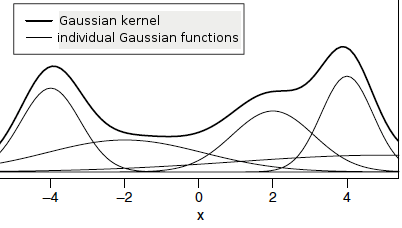
\includegraphics[scale=0.5]{gaussianKernel.png}
		\caption{Ejemplo de cinco funciones gaussianas y su superposición que es el núcleo resultante. Extraída de \cite{soc:dor}}
		\label{fig:gaussianKernel}
	\end{figure}

	Al usar ACO en problemas de optimización combinatoria, en cada iteración, al elegir una componente para ser agregada
	a la solución (de acuerdo a la ecuación (\ref{eq:chooseComponent})), una hormiga usa la información de las feromonas
	-almacenada como tabla- como una distribución de probabilidad discreta. En el caso continuo, la elección de la hormiga
	no está restringida a un conjunto finito. Por lo tanto, la información de las feromonas no puede almacenarse en una tabla
	y debe adoptarse un enfoque diferente.
	
	En ACO\textsubscript{$\mathbb{R}$}, se mantiene un registro de un número de soluciones dentro de un \textit{archivo} $T$. Para cada solución
	$s_l$ de un problema de $n$ dimensiones, ACO\textsubscript{$\mathbb{R}$} almacena en $T$ los valores de las $n$ variables y el valor de la
	función objetivo $f(s_l)$. De esta forma, la $i$-ésima variable de la $l$-ésima solución está denotada por $s_l^i$.
	
	La información almacenada en $T$ se utiliza luego para ir generando funciones de densidad de probabilidad dinámicamente. Como se
	indicó en la ecuación (\ref{eq:nucleoGauss}), el núcleo gaussiano $G^i$ está parametrizado por tres vectores $w$, $\mu$ y $\sigma$,
	cada uno con la misma cardinalidad. Las soluciones en el archivo $T$ se usan para calcular los valores de estos 
	tres parámetros y por consiguiente darle forma a la FDP del núcleo gaussiano usado para guiar a las hormigas en el proceso de búsqueda. El número de 	soluciones almacenadas en el archivo $T$ será $k$, la cardinalidad de cada uno de los vectores, y determina
	la complejidad de la FDP: habrá $k$ gaussianas individuales conformando el núcleo.
	
	Para cada variable del problema $i = 1, \dots, n$, hay una FDP definida por el núcleo $G^i$. Para cada uno de estos núcleos $G^i$,
	el vector $\mu^i$ se compone de los valores de la $i$-ésima variable de cada una de las soluciones en el archivo:
	\begin{equation}
	\mu^i = \{s^i_1, \dots, s^i_k \}
	\end{equation}
	
	El vector de pesos $w$, se crea de la siguiente forma: cada solución que se agrega al archivo $T$ se evalúa y puntúa (en caso de
	empate se define aleatoriamente). Las soluciones luego son ordenadas de acuerdo a su puntuación, es decir, la solución $s_l$ está
	$l$-ésima en el ranking. En el caso de un problema de minimización de una función $f$ como el que estamos tratando,  la puntuación
	de la solución $s_i$ está dada por $f(s_i)$ y, por lo tanto, será mejor mientras más bajo sea ese valor.
	El peso de la solución $s_l$ se calcula con la siguiente fórmula:
	\begin{equation}
	\label{eq:vectorPesos}
	\omega_l = \frac{1}{qk\sqrt{2\pi}}e^{-\frac{(l-1)^2}{2q^2k^2}}
	\end{equation}
	lo cual define que el peso es el valor de una gaussiana con argumento $l$, media $1$ y desviación estándar $qk$, donde $q$ es
	un parámetro del algoritmo. Cuando $q$ es pequeño, las soluciones mejor puntuadas son fuertemente preferidas, mientras que si es
	grande el algoritmo se vuelve más uniforme. La influencia de este parámetro en ACO\textsubscript{$\mathbb{R}$} es similar a ajustar el balance entre
	usar las estrategias de usar la mejor solución de la iteración o la mejor hallada hasta el momento para actualizar las feromonas en
	ACO. La figura (\ref{fig:archivo}) muestra la estructura del archivo $T$, el vector $w$ y los núcleos gaussianos.
	
	Para terminar de definir el núcleo $G^i$, resta determinar el vector de desviaciones estándar $\sigma^i$, lo cual haremos en la siguiente
	sección.
	
	\begin{figure}[h!]
		\centering
		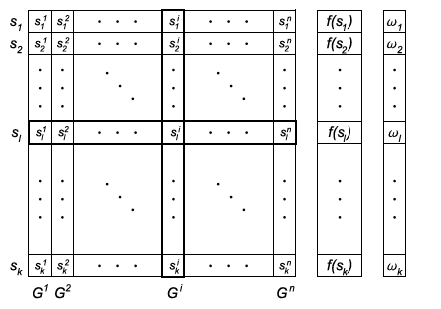
\includegraphics[scale=0.5]{archive.png}
		\caption{El archivo de soluciones utilizado por ACO\textsubscript{$\mathbb{R}$}. Las $k$ soluciones son ordenadas de acuerdo a su calidad.
		Es decir, para un problema de minimización, $f(s_1) \leq f(s_2) \leq \dots \leq f(s_k)$. Cada solución tiene asociado un peso
		proporcional a la calidad de la solución, es decir $w_1 \geq w_2 \geq \dots \geq w_k$. La FDP $G^i$ se construye utilizando solamente
		los $i$-ésimos valores de cada una de las $k$ soluciones.}
		\label{fig:archivo}
	\end{figure}
	
	\subsubsection{\textit{Implementación algorítmica de ACO\textsubscript{$\mathbb{R}$}}}
	En esta sección describiremos las actividades referidas en el algoritmo  \ref{alg:acoMetaheuristic} pero aplicadas a ACO\textsubscript{$\mathbb{R}$}.
	\bigbreak
	\textit{ConstruirSolución()}: Dadas las variables $x_i, i = 1, \dots, n$, una hormiga construye una solución realizando $n$ pasos de
	construcción. En el paso $i$, la hormiga escoge un valor para la variable $x_i$. Como se mencionó en la sección anterior, la FDP dada
	por el núcleo gaussiano está compuesta de un número dado de funciones gaussianas individuales. Dicho número es igual al tamaño
	$k$ del archivo $T$. En el paso $i$, sólo la información de la variable $x_i$ es utilizada. De este modo, en cada paso el núcleo $G^i$
	utilizado es diferente. De acuerdo a la ecuación (\ref{eq:nucleoGauss}), para poder definir $G^i$ los vectores $w$, $\mu^i$ y 
	$\sigma^i$ deben estar definidos. Si bien se ha explicado en la sección anterior cómo crear $w$ y $\mu^i$, el cálculo de 
	$\sigma^i$ es bastante más complejo. Antes de presentar cómo realizarlo, es conveniente explicar la implementación de la
	ecuación (\ref{eq:nucleoGauss}).
	
	En la práctica, el proceso de muestreo se realiza como sigue. Primero, los elementos del vector de pesos $w$ se computan de
	acuerdo a la ecuación (\ref{eq:vectorPesos}). Luego el proceso sigue en dos fases: en la primera se escoge alguna de las funciones
	gaussianas que componen el núcleo. La probabilidad $p_l$ de escoger la $l$-ésima gaussiana está dada por:
	\begin{equation*}
	p_l = \frac{w_l}{\sum_{r=1}^{k}w_r}
	\end{equation*}
	La segunda fase consiste en muestrear la gaussiana escogida (\textit{i.e}, en el paso $i$ la función $g_l^i$). Esto puede hacerse
	utilizando un generador de números aleatorios capaz de generar números aleatorios de acuerdo a una distribución normal
	parametrizada, o utilizando un generador aleatorio uniforme junto con, por ejemplo, el método de Box-Müller. Este muestreo de dos
	fases equivale a muestrear el núcleo $G^i$ definido en la ecuación (\ref{eq:nucleoGauss}).
	
	En el paso $i$, la desviación estándar necesita ser conocida únicamente para la gaussiana individual $g_l^i(x)$ escogida en la fase
	uno. Por lo tanto, no es necesario computar el vector completo $\sigma^i$, sino solamente la $\sigma^i_l$ requerida.
		
	Para establecer el valor de la desviación estándar $\sigma^i_l$ en el paso $i$, calculamos la distancia promedio de la solución
	escogida $s_l$ a las otras soluciones dentro del archivo $T$, y las multiplicamos por un parámetro $\xi$:
	\begin{equation*}
	\sigma^i_l = \xi \sum_{e=1}^{k}\frac{\abs{s^i_e - s^i_l}}{k-1}
	\end{equation*}
	El parámetro $\xi > 0$, que es el mismo para todas las variables, tiene un efecto similar al de la tasa 
	de evaporación en ACO. Mientras más alto sea su valor, más baja será la velocidad de convergencia del algoritmo.
	 
	Mientras que en ACO la tasa de evaporación afecta la memoria de largo plazo -\textit{i.e}, las peores soluciones son olvidadas más rápido-, $\xi$ en ACO\textsubscript{$\mathbb{R}$} afecta el modo en que la memoria de largo plazo es usada -\textit{i.e}, la búsqueda está menos influenciada hacia los puntos en el espacio de búsqueda que ya han sido explorados (y son mantenidos en el archivo $T$)-.
	\bigbreak	
	\textit{ActualizarFeromonas()}: Como se mencionó previamente, la información de feromonas en ACO\textsubscript{$\mathbb{R}$} se mantiene
	en el archivo de soluciones. Esto implica que el proceso de actualización de feromonas debe realizar alguna forma de actualización
	de dicho archivo.
	
	El tamaño $k$ del archivo $T$ es un parámetro del algoritmo. Sin embargo, $k$ no puede ser menor que el número de variables
	del problema que se intenta resolver \cite{soc:dor}.
	
	Al comenzar el algoritmo, el archivo de soluciones $T$ se inicializa generando $k$ soluciones mediante un muestreo aleatorio uniforme.
	La actualización de feromonas se consigue agregando el conjunto de nuevas soluciones generadas al archivo $T$ y luego eliminando
	el mismo número de peores soluciones de forma que el tamaño de $T$ no cambie. Este proceso garantiza que sólo las mejores
	soluciones son mantenidas en el archivo, guiando efectivamente a las hormigas en el proceso de búsqueda.
	\bigbreak
	\textit{AccionesDaemon()}: Se va actualizando la mejor solución encontrada hasta el momento de forma que pueda ser devuelta
	una vez que se alcanzan las condiciones de terminación. Se podrían aplicar heurísticas de búsqueda local para 
	mejorar la \textit{performance} del algoritmo.
	
	\section{\textbf{ACO\textsubscript{$\mathbb{R}$} Aplicado al Problema del Filtro}}
	En esta sección detallamos la implementación de la metaheurística ACO\textsubscript{$\mathbb{R}$} 
	para resolver el problema del filtro especificado en la sección (\ref{sec:fundelect}).
	
	En la sección \ref{subsec:VersionContinua} presentamos primero el caso en que todas las variables 
	son libres y reales para ver la convergencia del algoritmo.  En la sección \ref{subsec:VersionContinuaR1Fijado}
	modificamos ligeramente el algoritmo para que el valor de $R_1$ quede fijo a alguno de los valores admisibles definidos por la serie $E$ 
	y analizamos las soluciones continuas obtenidas.
	
	A continuación, en la sección \ref{subsec:VersionDiscreta}, extendemos el algoritmo de la sección anterior
	para que, una vez obtenida la solución para variables continuas, 
	realice una búsqueda entre los vecinos discretos más cercanos a esa solución de variables continuas.
	
	Luego, en la sección \ref{subsec:VersionDiscretaPura}, introducimos una modificación al algoritmo 
	ACO\textsubscript{$\mathbb{R}$} para que trabaje con valores discretos. 
	Finalmente, veremos que si $R_1$ se deja libre, la versión discreta no encuentra buenas soluciones en general.
	
	Para cada una de las variantes, definimos una única función \textit{costo} que es el objetivo a minimizar y, por lo tanto, 
	será la ultima columna	de cada entrada del archivo de soluciones. A continuación el pseudocódigo muestra la 
	función costo utilizada en todos los casos.
	\newpage
	\begin{breakablealgorithm}
		\caption{Función costo a minimizar}
	    \begin{algorithmic}[1]
	    	\State $R_{min}, R_{max}$: Valores mínimo y máximo que pueden tomar las resistencias
	    	\State $C_{min}, C_{max}$: Valores mínimo y máximo que pueden tomar los capacitores
	    	\State $W_G \gets 10000$: Peso de la restricción sobre la ganancia
	    	\State $W_\omega \gets 10$: Peso de la restricción sobre $\omega$
	    	\State $W_Q \gets 10$: Peso de la restricción sobre $Q$
	    	\State $W_S \gets 100$: Peso de la restricción sobre la sensibilidad
	    	\State $W_{Max}  \gets 1\mathrm{e}{11}$: Penalización para variables fuera de rango
	    	\State $G_{obj} \gets 3$: Ganancia objetivo
	    	\State $\omega_{obj} \gets 2000 * \pi$: Frecuencia de polo objetivo
	    	\State $Q_{obj} \gets 0.707$: Factor de calidad objetivo
	    	
	    	\item[]
	    	
	    	\Function{EnRango}{Comp}
	    	\If{$\Call{EsResistencia}{Comp}$}
	    		\State \Return $R_{min} < Comp < R_{max}$
	    	\Else
	    		\State \Return $C_{min} < Comp < C_{max}$
	    	\EndIf
	    	\EndFunction
	    	
	    	\item[]
	    	
	    	\Function{Costo}{$R_1$, $R_2$, $R_3$, $C_4$, $C_5$}
	    		\State $RangosOK \gets \bigl<\forall\ c: c \in \lbrace R_1, R_2, R_3, C_4, C_5 \rbrace: \Call{EnRango}{c} \bigr>$
	    		\If{$RangosOK$}
	    			\State $Sens \gets \Call{Sensibilidad}{R_1, R_2, R_3, C_4, C_5}$
	    			\State $Q \gets \Call{FactorCalidad}{R_1, R_2, R_3, C_4, C_5}$
	    			\State $G \gets \Call{Ganancia}{R_1, R_2, R_3, C_4, C_5}$
	    			\State $\omega \gets \Call{FrecuenciaPolo}{R_1, R_2, R_3, C_4, C_5}$
	    			\State $Costo \gets W_S * Sens^2 + W_G * (G - G_{obj})^2 + W_\omega * (\log (\omega / \omega_{obj}))^2 + W_Q *(\log (Q / Q_{obj})^2)$
	    			\State \Return $Costo$
	    		\Else
	    			\State \Return $W_{Max}$
	    		\EndIf
	    	\EndFunction
	    \end{algorithmic}
    \end{breakablealgorithm}

	
	
	\subsection{Versión continua con todas las variables libres}
	\label{subsec:VersionContinua}
	En esta primera versión del algoritmo el dominio de las variables es todo el intervalo continuo entre los valores
	admisibles máximos y mínimos especificados por las series $E$. Es conveniente que definamos algunas funciones 
	elementales aquí para hacer el pseudocódigo más 
	legible \footnote{Estas funciones pueden encontrarse ya implementadas en varias librerías o lenguajes como 
	por ejemplo \textit{Python} -en la librería \textit{Numpy}- y \textit{Matlab}}. 

	\begin{itemize}
		\item $zeros(n)$: devuelve un arreglo $A$ de n elementos, todos inicializados en 0.
		\item $zeros (m, n)$: devuelve una matriz M de tamaño $m \times n$ con todos sus elementos inicializados en 0.
		\item $repmat(M, f, c)$: dada una matriz $M$ devuelve una matriz que replica $f$ copias de $M$ en las filas y $c$ copias en las
		columnas.
		\item $randUniform(m, n)$: dados $m < n$ devuelve un número aleatorio con distribución uniforme en el intervalo
		 $[m,n]$. Si $m$ y $n$ se omiten, toman por defecto el valor 0 y 1 respectivamente. 
		\item $randn()$: Devuelve un valor aleatorio correspondiente a una distribución de probabilidad normal estándar.
		\item $cumsum(p)$:
		\item $sort(M, c)$: ordena las filas de la matriz $M$ de menor a mayor de acuerdo al valor de la columna $c$.
		\item $concat(M,N)$: dadas las matrices $M$ de tamaño $m \times n$ y $N$ de tamaño $l \times n$ devuelve una matriz $M'$
		de tamaño $(m+l) \times n$ donde
		\begin{equation*}
		M'[i][j] =
		\begin{cases}
		M[i][j],& \text{si } i \leq m\\
		N[l+(i-m-1)][j],              & \text{caso contrario}
		\end{cases}
		\end{equation*}
		\item $sum(A)$: Dado un arreglo numérico $A$, devuelve la suma de sus elementos. 
	\end{itemize}
	
	El pseudocódigo correspondiente a esta versión puede verse a continuación:
	\begin{breakablealgorithm}
%		\begin{algorithm}[H]
		\caption{ACO\textsubscript{$\mathbb{R}$} Continuo Libre}
		\label{alg:continuoLibre}
		\begin{algorithmic}[1]
			\State $R_{min}, R_{max}$: Valores mínimo y máximo que pueden tomar las resistencias
			\State $C_{min}, C_{max}$: Valores mínimo y máximo que pueden tomar los capacitores 
			\State $TamArchivo$: cantidad de soluciones que se mantienen en el archivo $T$
			\State $TamMuestra$: cantidad de hormigas que se lanzan por iteración
			\State $NumIt$: número de iteraciones
			\State $FactorIntensidad$: $\xi$
			\State $NumVars = 5$ \Comment{$R_1, R_2, R_3, C_4, C_5$}
			\State $zeta$: Deviation Distance Ratio
						
			\item[]
			\Function{ElegirNucleo}{p}
			\State $r \gets randUniform()$
			\State $C \gets cumsum(p)$
			\State \Return $\bigl<Min\ j: 0 \leq j <size(C): C[j] > r \bigr>$
			\EndFunction
			
			\item[]
			
			\Procedure{InicializarArchivo}{$T$} \Comment{Inicializa aleatoriamente el archivo}
			\For{cada fila $f$ en $T$}
			\State $f[0\dots2] \gets randUniform(R_{min}, R_{max})$
			\State $f[3\dots4] \gets randUniform(C_{min}, C_{max})$
			\State $f[5] \gets \Call{Costo}{f[0\dots4]}$
			\EndFor
			\EndProcedure
			
			\item[]
			
			\Function{HallarSoluciones}{}()
			\State $fila \gets zeros(NumVars+1)$
			\State $T \gets repmat(fila, TamArchivo, 1)$
			\State \Call{InicializarArchivo}{$T$}
			\State $sort(T, NumVars)$
			\State $w \gets zeros(TamArchivo)$ \Comment{Arreglo con los pesos}
			\For{$l$ en $\lbrack 0 \dots TamArchivo \rparen$}
			\State $b \gets  \frac{1}{\sqrt{2\pi} \cdot FactorIntensidad \cdot TamArchivo}$
			\State $c \gets e^{-\frac{l}{2 \cdot (FactorIntensidad \cdot TamArchivo)^2}}$
			\State $w[l] \gets b \cdot c $ 
			\EndFor
			\State $p \gets zeros(TamArchivo)$ \Comment{Arreglo con las probabilidades}
			\For{$l$ en $\lbrack 0 \dots TamArchivo \rparen$ }
			\State $p[l] \gets \frac{w[l]}{sum(w)}$
			\EndFor
			\item[]
			\For{$it$ en $\lbrack 0 \dots NumIt\rparen$} \Comment{Loop principal}
			\State $\mu \gets zeros(TamArchivo, NumVars)$ \Comment{Arreglo con las medias}
			\For{$j$ en $\lbrack 0 \dots TamArchivo \rparen$}
			\State $\mu[j] \gets T[j][0 \dots NumVars - 1]$
			\EndFor
			\State $\sigma \gets zeros(TamArchivo, NumVars)$ \Comment{Arreglo con las desv. est.}
			\For{$j$ en $\lbrack 0 \dots TamArchivo \rparen$}
			\State $D \gets \sum_{r=0}^{TamArchivo - 1}\abs{\mu[j]-\mu[r]}$
			\State $\sigma[j] \gets \frac{zeta * D}{TamArchivo -1}$
			\EndFor
			\item[]
			\State $NuevaPobl \gets repmat(fila, TamMuestra, 1)$
			\For{$t$ en $\lbrack 0 \dots TamMuestra \rparen$}
			\State $NuevaPobl[t]\lbrack 0 \dots NumVars \rparen \gets zeros(NumVars)$
			\For{$i$ en $\lbrack 0 \dots NumVars \rparen$}
			\State $g \gets$ \Call{ElegirNucleo}{p} \Comment{Escoger núcleo Gaussiano}
			\State $NuevaPobl[t][i] \gets \mu[g][t] + \sigma[g][i] \cdot rand()$
			\EndFor
			\State $NuevaPobl[t][NumVars] \gets$ \Call{Cost}{$NuevaPobl \lbrack 0 \dots NumVars \rparen$}
			\EndFor
			\State $PobTotal \gets concat(T, NuevaPobl)$
			\State $sort(PobTotal, NumVars)$
			\State $T \gets PobTotal \lbrack 0 \dots TamArchivo \rparen$ \Comment{Actualizar archivo con las mejores soluciones}
			\EndFor
			\State $Sol \gets Archivo[0]$
			\State \Return $Sol$
			\EndFunction
		\end{algorithmic}
%	\end{algorithm}
	\end{breakablealgorithm}

	Es dable notar que hemos utilizado dos variantes del algoritmo: en la primera el muestreo y selección de las variables 
	se hace directamente sobre su valor, mientras que en la segunda se hace utilizando el logaritmo de los valores. Esta 
	diferenciación se hace efectiva en el algoritmo simplemente modificando el procedimiento de inicialización del archivo donde
	se cambian los límites de la llamada a \textit{randUniform} utilizando $\log(R_{min})$ y $\log(R_{max})$ -lo mismo se hace
	con los capacitores-. Los resultados obtenidos con la versión logarítmica fueron sensiblemente mejores, como puede observarse
	en el cuadro \ref{cuadroSols1}.
	
	Además, en las figuras (\ref{fig:F-r1}), (\ref{fig:F-c4}), (\ref{fig:F-r2}), (\ref{fig:F-c5}), (\ref{fig:F-r3}) y (\ref{fig:F-costo}) 
	podemos visualizar la convergencia de la función costo así como también de las cinco variables para la versión logarítmica.
	
	La implementación en \textit{Python} del algoritmo \ref{alg:continuoLibre} puede verse en el apéndice \ref{subsec:pythoncontinuo}.
	
	\begin{table}[!h]
		$$
		\begin{array}{|c|c|c|}
		\hline
		 & Com\acute{u}n & Logar\acute{\imath}tmica \\
                \hline
                R1 & 143119.89  & 3561.17 \\
                R2 & 429268.55 & 10683.34 \\
                R3 & 107334.23  & 2671.14 \\
                C4 & 2.10*10^{-9}  & 8.43*10^{-8}\\
                C5 & 1.00*10^{-9} & 1.05*10^{-8}\\
                Costo & 65.209 &  56.248\\
                Sens & 0.75 & 0.75 \\
                ErrG & 0.021\%  & 0.016\%\\
                ErrO & 48.794\%  &  0.002\%\\
                ErrQ & 48.801\%  &  0.005\%\\
		\hline
		\end{array}
		$$
		\caption{Resultados obtenidos con la versión común y logarítmica para la variante continua con todas las variables libres.}
		\label{cuadroSols1}
	\end{table}
	
	\begin{figure}[!h]                                                                                  
		\centering                                                                                      
		\begin{subfigure}{0.5\textwidth}
			\centering
			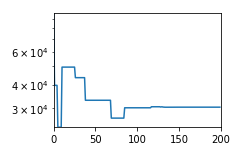
\includegraphics[scale=0.7]{ContinuoLibre/cc-r1}
			\caption{}
			\label{fig:F-r1}
		\end{subfigure}%
		\begin{subfigure}{0.5\textwidth}
			\centering
			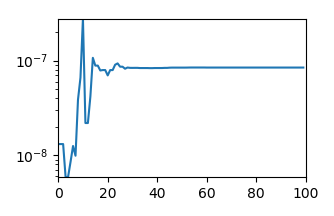
\includegraphics[scale=0.7]{ContinuoLibre/cc-c4}
			\caption{}
			\label{fig:F-c4}
		\end{subfigure}   \\                                                         
		\begin{subfigure}{0.5\textwidth}
			\centering
			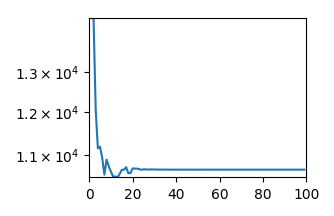
\includegraphics[scale=0.7]{ContinuoLibre/cc-r2}
			\caption{}
			\label{fig:F-r2}
		\end{subfigure}%
		\begin{subfigure}{0.5\textwidth}
			\centering
			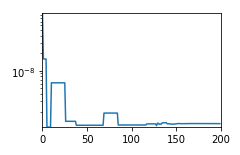
\includegraphics[scale=0.7]{ContinuoLibre/cc-c5}
			\caption{}
			\label{fig:F-c5}
		\end{subfigure}   \\                                                         
		\begin{subfigure}{0.5\textwidth}
			\centering
			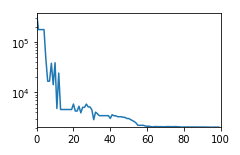
\includegraphics[scale=0.7]{ContinuoLibre/cc-r3}
			\caption{}
			\label{fig:F-r3}
		\end{subfigure}%
		\begin{subfigure}{0.5\textwidth}
			\centering
			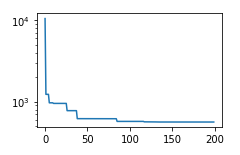
\includegraphics[scale=0.7]{ContinuoLibre/cc-costo}
			\caption{}
			\label{fig:F-costo}
		\end{subfigure}                                                            
		\caption{Convergencia de las distintas variables y la función costo para la versión continua con todas las variables libres. El eje vertical 
			corresponde al valor de la variable y el horizontal al número de iteración. (a) R1, (b) C4, (c) R2, (d) 
			C5, (e) R3 y (f) costo. }                                                                                  
		\label{fig:FF}                                                                                  
	\end{figure}
	
	\subsection{Versión continua con $R_1$ fijado}
	\label{subsec:VersionContinuaR1Fijado}
	En la sección \ref{subsec:VersionContinua} vimos cómo ACO\textsubscript{$\mathbb{R}$} converge hacia valores dentro 
	del rango continuo que cada componente puede tomar, a la vez que minimiza la función costo. Sin embargo, 
	en nuestro problema, el conjunto de valores que puede tomar cada componente del filtro proviene de un conjunto finito. 
	En esta sección modificamos ligeramente el algoritmo (\ref{alg:continuoLibre}) de forma que iteramos sobre cada valor 
	que puede tomar $R_1$ y obtenemos una solución continua utilizando la función \textbf{HallarSoluciones}. 
	En este caso, el número de variables $NumVars$ pasa a ser  4 en vez de 5, ya que R1 queda fijado.
	
	Como en la sección \ref{subsec:VersionContinua} tendremos una versión que trabaja directamente
	con los valores de los componentes y otra que lo hace con los logaritmos. El pseudocódigo -donde omitimos
	redefinir aquellos parámetros que son los mismos que en el algoritmo \ref{alg:continuoLibre}- se muestra a continuación.
	
	\begin{breakablealgorithm}
		\caption{ACO\textsubscript{$\mathbb{R}$} continuo con $R_1$ fijo}
		\label{alg:continuoFijo}
		\begin{algorithmic}[1]
			\State $NumVars = 4$ \Comment{$R_2, R_3, C_4, C_5$}
			\State $Soluciones \gets []$
			\For{$R_1$ en $ValoresResistencias$}
				\State $Sol \gets [R_1] +  \Call{HallarSoluciones}{}()$ \Comment{Función definida en algoritmo \ref{alg:continuoLibre}}
				\State Agregar $Sol$ a la lista $Soluciones$
			\EndFor
		\end{algorithmic}
	\end{breakablealgorithm}

	A modo de ejemplo, incluimos en los cuadros \ref{cuadroSolsExh}, \ref{cuadroSolsCom} y \ref{cuadroSolsLog} los 
	resultados para los mejores 5 valores de $R_1$ de acuerdo a las soluciones obtenidas mediante el algoritmo exhaustivo
	de la sección \ref{sec:AlgoritmoExhaustivo}, para la versión exhaustiva, la que trabaja directamente con los valores 
	de las variables y para aquella que lo hace con los logaritmos, respectivamente.
	
	\begin{table}[!h]
		$$
		\begin{array}{|c|c|c|c|c|c|c|c|c|c|}
		\hline
		R_1 & R_2 & R_3 & C_4 & C_5 & Sens & Err_G & Err_\omega & Err_Q \\
		\hline
		11000 & 33000 & 8200 & \expnumber{2.7}{-8} & \expnumber{3.3}{-9} & 0.7508 & 0\% & 2.499\% & 1.145\% \\
		3600 & 11000 & 2700 & \expnumber{8.2}{-8} & \expnumber{1}{-8} & 0.7540 & 1.852\% & 1.985\% & 0.561\% \\
		36000 & 110000 & 27000 & \expnumber{8.2}{-9} & \expnumber{1}{-9} & 0.7540 & 1.852\% & 1.985\% & 0.561\% \\
		12000 & 36000 & 8200 & \expnumber{2.7}{-8} & \expnumber{3.3}{-9} & 0.7616 & 0\% & 1.865\% & 1.036\% \\
		3300 & 10000 & 2200 & \expnumber{1}{-7} & \expnumber{1.2}{-8} & 0.7668 & 1.010\% & 2.047\% & 1.510\% \\
		\hline
		\end{array}
		$$
		\caption{Resultados obtenidos con la versión exhaustiva.}
		\label{cuadroSolsExh}
	\end{table}

	\begin{table}[!h]
		$$
		\begin{array}{|c|c|c|c|c|c|c|c|c|c|}
		\hline
		R_1 & R_2 & R_3 & C_4 & C_5 & Sens & Err_G & Err_\omega & Err_Q \\
		\hline
		11000 & 33000 & 8246.68 & \expnumber{2.73}{-8} & \expnumber{3.41}{-9} & 0.75 & 0\% & 0.022\% & 0.011\% \\
		3600 & 10800 & 2700 & \expnumber{8.34}{-8} & \expnumber{1.04}{-8} & 0.75 & 0\% & 0\% & 0\% \\
		36000 & 108000 & 27000 & \expnumber{8.34}{-9} & \expnumber{1.04}{-9} & 0.75 & 0\% & 0\% & 0\% \\
		12000 & 36000.15 & 8992.27 & \expnumber{2.5}{-8} & \expnumber{3.12}{-9} & 0.7501 & 0\% & 0.060\% & 0.081\% \\
		3300 & 9900 & 2474.84 & \expnumber{9.09}{-8} & \expnumber{1.14}{-8} & 0.75 & 0\% & 0.001\% & 0\% \\
		\hline
		\end{array}
		$$
		\caption{Resultados obtenidos fijando $R_1$ y dejando el resto de las variables libres.}
		\label{cuadroSolsCom}
	\end{table}

	\begin{table}[!h]
		$$
		\begin{array}{|c|c|c|c|c|c|c|c|c|c|}
		\hline
		R_1 & R_2 & R_3 & C_4 & C_5 & Sens & Err_G & Err_\omega & Err_Q \\
		\hline
		11000 & 33000 & 8247.12 & \expnumber{2.73}{-8} & \expnumber{3.41}{-9} & 0.75 & 0\% & 0.012\% & 0.018\% \\
		3600 & 10800.02 & 2695.4 & \expnumber{8.35}{-8} & \expnumber{1.04}{-8} & 0.7502 & 0\% & 0.017\% & 0.005\% \\
		36000 & 107999.95 & 26923.72 & \expnumber{8.36}{-9} & \expnumber{1.04}{-9} & 0.7503 & 0\% & 0.097\% & 0.019\% \\
		12000 & 36000 & 8994 & \expnumber{2.5}{-8} & \expnumber{3.13}{-9} & 0.7501 & 0\% & 0.020\% & 0.055\% \\
		3300 & 9900.01 & 2474.33 & \expnumber{9.10}{-8} & \expnumber{1.14}{-8} & 0.75 & 0\% & 0.010\% & 0.016\% \\
		\hline
		\end{array}
		$$
		\caption{Resultados obtenidos fijando $R_1$ y dejando el resto de las variables libres. Versión logarítmica.}
		\label{cuadroSolsLog}
	\end{table}
	
	\subsection{Versión continua con búsqueda de vecinos discretos cercanos}
	\label{subsec:VersionDiscreta}
	Como vimos en la sección \ref{subsec:VersionContinuaR1Fijado}, las soluciones continuas obtenidas por ACO\textsubscript{$\mathbb{R}$} 
	si se fija $R_1$ son realmente buenas. Sin embargo, dichas soluciones  tienen valores para $R_2$, $R_3$, $C_4$ y $C_5$ que, 
	en general, no corresponden a los valores permitidos en las series industriales; pero a partir de esta solución podemos efectuar 
	una búsqueda de los vecinos más cercanos (por encima y por debajo) en la lista de valores permitidos para cada 
	componente. Inicialmente, la búsqueda se limito a los vecinos inmediatamente más cercanos, sin embargo las soluciones obtenidas
	no resultaron demasiadas y decidimos extender la búsqueda a 2 vecinos, tanto por arriba como por debajo. Así mismo también
	se decidió incluir a $R_1$ en la búsqueda de vecinos para extender un poco el espacio de búsqueda local. Cabe destacar que aquí
	también hemos trabajado con una versión logarítmica pero sin embargo las soluciones obtenidas fueron las mismas.
	
	Los resultados se muestran en el cuadro \ref{cuadroSolVecinos}. En el algoritmo \ref{alg:vecinos} se muestra el pseudocódigo y el 
	código \textit{Python} puede verse en el apéndice \ref{subsec:pythondiscreto}.
	
	\begin{table}[H]
		$$
		\begin{array}{|c|c|c|c|c|c|c|c|c|c|}
		\hline
		R_1 & R_2 & R_3 & C_4 & C_5 & Err_G & Err_Q & Err_{\omega_p} & Sens & \text{B\'usq. ext.}   \\
		\hline
		1300 & 3900 & 1100 & \expnumber{2.2}{-7} & \expnumber{2.7}{-8} & 0\% & 0.74\% & 0.3\% & 0.795 & \textbf{X} \\
		1600 & 4700 & 1300 & \expnumber{1.8}{-7} & \expnumber{2.2}{-8} & 2.08\% & 1.84\% & 2.32\% & 0.778 & \textbf{X} \\
		2700 & 8200 & 1800 & \expnumber{1.2}{-7} & \expnumber{1.5}{-8} & 1.23\% & 0.64\% & 2.36\% & 0.767 & \textbf{X} \\
		2700 & 8200 & 2700 & \expnumber{1}{-7} & \expnumber{1.2}{-8} & 1.23\% & 0.57\% & 2.36\% & 0.859 & \textbf{X} \\
		3000 & 9100 & 2400 & \expnumber{1}{-7} & \expnumber{1.2}{-8}  & 1.11\% & 1.59\% & 1.69\% & 0.775 &  \\
		3300 & 10000 & 2200 & \expnumber{1}{-7} & \expnumber{1.2}{-8} & 1.01\% & 1.49\% & 2.05\% & 0.767 & \textbf{X} \\
		3300 & 10000 & 3000 & \expnumber{8.2}{-8} & \expnumber{1}{-8} & 1.01\% & 0.41\% & 1.47\% & 0.823 & \textbf{X} \\
		3600 & 11000 & 2700 & \expnumber{8.2}{-8} & \expnumber{1}{-8}  & 1.85\% & 0.55\% & 1.98\% & 0.754 & \\
		4300 & 13000 & 2400 & \expnumber{8.2}{-8} & \expnumber{1}{-8} & 0.78\% & 0.16\% & 0.5\% & 0.788 & \textbf{X} \\
		4300 & 13000 & 3600 & \expnumber{6.8}{-8} & \expnumber{8.2}{-9} & 0.78\% & 1.37\% & 1.48\% & 0.792 & \\
		5100 & 15000 & 3000 & \expnumber{6.8}{-8} & \expnumber{8.2}{-9} & 1.96\% & 1.85\% & 0.47\% & 0.776 & \textbf{X} \\
		5100 & 15000 & 4300 & \expnumber{5.6}{-8} & \expnumber{6.8}{-9} & 1.96\% & 2.02\% & 1.55\% & 0.792 & \textbf{X} \\
		6800 & 20000 & 6800 & \expnumber{3.9}{-8} & \expnumber{4.7}{-9} & 1.96\% & 1.51\% & 0.8\% & 0.855 & \textbf{X} \\
		7500 & 22000 & 4300 & \expnumber{4.7}{-8} & \expnumber{5.6}{-9} & 2.22\% & 2.4\% & 0.86\% & 0.779 & \textbf{X} \\
		9100 & 27000 & 5100 & \expnumber{3.9}{-8} & \expnumber{4.7}{-9} & 1.1\% & 1.21\% & 0.18\% & 0.784 & \textbf{X} \\
		10000 & 30000 & 9100 & \expnumber{2.7}{-8} & \expnumber{3.3}{-9} & 0\% & 0.66\% & 2.05\% & 0.822 & \\
		11000 & 33000 & 6200 & \expnumber{3.3}{-8} & \expnumber{3.9}{-9} & 0\% & 1.8\% & 1.92\% & 0.785 & \textbf{X} \\
		11000 & 33000 & 8200 & \expnumber{2.7}{-8} & \expnumber{3.3}{-9}  & 0\% & 1.13\% & 2.49\% & 0 .751&\\
		12000 & 36000 & 8200 & \expnumber{2.7}{-8} & \expnumber{3.3}{-9}  & 0\% & 1.02\% & 1.87\% & 0.762 & \\
		13000 & 39000 & 7500 & \expnumber{2.7}{-8} & \expnumber{3.3}{-9} & 0\% & 0.27\% & 1.41\% & 0.783 & \textbf{X} \\
		13000 & 39000 & 11000 & \expnumber{2.2}{-8} & \expnumber{2.7}{-9} & 0\% & 0.74\% & 0.3\% & 0.795 & \textbf{X} \\
		16000 & 47000 & 13000 & \expnumber{1.8}{-8} & \expnumber{2.2}{-9} & 2.08\% & 1.84\% & 2.32\% & 0.778 & \textbf{X} \\ 
		27000 & 82000 & 18000 & \expnumber{1.2}{-8} & \expnumber{1.5}{-9} & 1.23\% & 0.64\% & 2.36\% & 0.767 & \textbf{X} \\ 
		27000 & 82000 & 27000 & \expnumber{1}{-8} & \expnumber{1.2}{-9} & 1.23\% & 0.57\% & 2.36\% & 0.859 & \textbf{X} \\
		30000 & 91000 & 24000 & \expnumber{1}{-8} & \expnumber{1.2}{-9}  & 1.11\% & 1.59\% & 1.69\% & 0.775 & \\
		33000 & 100000 & 22000 & \expnumber{1}{-8} & \expnumber{1.2}{-9} & 1.01\% & 1.49\% & 2.05\% & 0.767 & \textbf{X} \\
		33000 & 100000 & 30000 & \expnumber{8.2}{-9} & \expnumber{1}{-9} & 1.01\% & 0.41\% & 1.47\% & 0.823 & \textbf{X} \\
		36000 & 110000 & 27000 & \expnumber{8.2}{-9} & \expnumber{1}{-9}  & 1.85\% & 0.55\% & 1.98\% & 0.754 & \\
		43000 & 130000 & 24000 & \expnumber{8.2}{-9} & \expnumber{1}{-9} & 0.78\% & 0.16\% & 0.5\% & \textbf{X} \\
		\hline
		\end{array}
		$$
		\caption{Soluciones obtenidas con búsqueda de vecinos discretos. En la última columna se marca con una \textbf{X} aquellas
		soluciones que fueron halladas extendiendo el rango de búsqueda a 2 vecinos.}
		\label{cuadroSolVecinos}
	\end{table}
	
	
	\begin{breakablealgorithm}
		\caption{ACO\textsubscript{$\mathbb{R}$} Discreto con Búsqueda de Vecinos Cercanos}
		\label{alg:vecinos}
		\begin{algorithmic}[1]
			\State $G^{max}, G^{min}$: Valores máximo y mínimo aceptables para la ganancia
			\State $\omega_p^{max}, \omega_p^{min}$: Valores máximo y mínimo aceptables para la frecuencia de polo
			\State $Q_p^{max}, Q_p^{min}$: Valores máximo y mínimo aceptables para el factor de calidad
			\State $Soluciones \gets []$
			\For{$R_1$ en $ValoresResistencias$}
				\State $Sol \gets [R_1] +  \Call{HallarSoluciones}{}()$ \Comment{Función definida en el algoritmo \ref{alg:continuoLibre}}
				\State $Vecinos \gets []$
				\For{$Componente$ en $Sol$} \Comment{Buscar vecinos de cada componente}
					\State $(V_l, V_r) \gets VecinosCercanos(Componente, PosiblesValores)$
					\State Agregar $(V_l, V_r)$ a la lista $Vecinos$
				\EndFor
				\For{$r_1$ en $Vecinos[0]$}
				\For{$r_2$ en $Vecinos[1]$}
				\For{$r_3$ en $Vecinos[2]$}
				\For{$c_4$ en $Vecinos[3]$}
				\For{$c_5$ en $Vecinos[4]$}
				\State $SolTentativa \gets  [r_1, r_2, r_3, c_4, c_5]$
				\State $Sens \gets $ \Call{Sensibilidad}{$SolTentativa$}
				\State $G \gets $ \Call{Ganancia}{$SolTentativa$}
				\State $Q_p \gets $ \Call{FactorCalidad}{$SolTentativa$}
				\State $\omega_p \gets $ \Call{FrecuenciaPolo}{$SolTentativa$}
				\State $G^{ok} \gets G^{min} < G < G^{max}$
				\State $Q_p^{ok} \gets Q_p^{min} < Q_p < Q_p^{max}$
				\State $\omega_p^{ok} \gets \omega_p^{min} < \omega_p < \omega_p^{max}$
				\If{$Sens < 1 \wedge G^{ok} \wedge \omega_p^{ok}  \wedge Q_p^{ok} $}
					\State Agregar $SolTentativa$ a la lista $Soluciones$
				\EndIf
				\EndFor
				\EndFor
				\EndFor
				\EndFor
				\EndFor
			\EndFor
		\end{algorithmic}
	\end{breakablealgorithm}

	\subsection{Versión Discreta \textit{Pura}}
	\label{subsec:VersionDiscretaPura}
	Para finalizar, presentamos ahora una variante donde, en vez de \textit{discretizar} las soluciones continuas encontradas por el algoritmo
	una vez que el mismo finaliza, se discretiza el valor de la componente seleccionada en cada paso de la iteración seleccionando
	el valor discreto posible más cercano al continuo generado. Como en las variantes anteriores, trabajaremos con una versión logarítmica también.
	Esta variante ha sido la que peor resultados ofrece ya que, en general, son necesarias varias corridas para que encuentre una solución adecuada.
	Presentamos a modo de ejemplo una tabla, tanto para la versión común como la logarítmica, con los 5 mejores valores de $R_1$ de acuerdo 
	a la solución exhaustiva,  junto al número de corridas necesarias hasta encontrar solución y la solución hallada. En el apéndice presentamos los
	resultados para todos los valores de $R_1$.
	
	\begin{table}[!h]
		$$
		\begin{array}{|c|c|c|c|}
		\hline
		R_1 & \text{Sol. Exhaustiva} & \text{Sol. Algorítmica} & \text{Corridas necesarias} \\
		\hline
		11000 & [11000; 33000; 8200; \expnumber{2.7}{-8}; \expnumber{3.3}{-9}] & \text{La misma} & 1 \\
		3600 & [3600; 11000; 2700; \expnumber{8.2}{-8}; \expnumber{1}{-8}] & \text{La misma} & 5 \\
		36000 & [36000; 110000; 27000; \expnumber{8.2}{-9}; \expnumber{1}{-9}] & [36000; 110000; 20000; \expnumber{1}{-8}; \expnumber{1.2}{-9}] & 30  \\
		12000 & [12000; 36000; 8200; \expnumber{2.7}{-8};\expnumber{3.3}{-9}] & \text{La misma} & 2  \\
		3300 & [3300; 10000; 2200; \expnumber{1}{-7}; \expnumber{1.2}{-8}] & \text{La misma} & 1  \\
		\hline
		\end{array}
		$$
		\caption{Resultados obtenidos con la versión discreta pura.}
		\label{cuadroSolDiscretoPuro}
	\end{table}
		

	\appendix
	\section{\textbf{Tablas de Resultados}}
	\subsection{Algoritmo Exhaustivo}
	\label{subsec:Resultados Exhaustivo}
	\subsection{Versión Continua}
	\label{subsec:Resultados Continuos}
	
	\section{\textbf{Código Python}}
	\subsection{Algoritmo Exhaustivo}
	\label{subsec:pythonexhaustivo}
	\inputminted{python}{exhaustivo.py}
	\subsection{Versión Continua}
	\label{subsec:pythoncontinuo}
	\inputminted{python}{filtro_continuoLibre.py}
	\subsection{Versión Discreta}
	\label{subsec:pythondiscreto}
	
  \begin{thebibliography}{1}
      \bibitem{corr}
      Corral, C.: 
      Designing RC active filters with standard-component values. Electronic Design
      Network Magazine, 141-154 (2000)
      
      \bibitem{lov:rom:per}
      Lovay, M., Romero, E., Peretti, M.:
      Diseño de Filtros Activos Robustos usando Algoritmos Genéticos.
      SII 2015 4$^\circ$ Simposio Argentino de Informática Industrial.
      
      \bibitem{dim}
      Dimopoulos, H.: 
      Analog Electronics Filters: Theory, Design and Synthesis. 
      Springer (2012)
      
      \bibitem{rau:swa}
      Raut, R., Swamy, M. N. S.: 
      Modern Analog Filter Analysis and Design: A Practical Approach. 
      Wiley-VCH (2010).
      
      \bibitem{sol}
      Solnon, C.:
      Ant Colony Optimization and Constraint Programming. (Wiley-ISTE 2010) 
      
      \bibitem{soc:dor}
      Socha, K., Dorigo, M.:
      Ant colony optimization for continuous domains.
      European Journal of Operational Research 185 (2008)
      
      \bibitem{dor92}
      Dorigo, M.:
      Optimization, Learning and Natural Algorithms (en italiano). 
      Ph.D. thesis, Dipartimento di Elettronica, Politecnico di Milano, Italy (1992).
      
      \bibitem{dor:man:col}
      Dorigo, M., Maniezzo, V., Colorni, A.: 
      Ant System: Optimization by a colony of cooperating agents. 
      IEEE Transactions on Systems, Man, and Cybernetics – Part B 26 (1), 29–41. (1996)
      
      \bibitem{stu:dor}
      Stützle, T., Dorigo, M.:
      ACO algorithms for the traveling salesman problem. 
      En: Miettinen, K., Mäkelä, M.M., Neittaanmäki, P., Périaux, J. (Eds.), Evolutionary Algorithms in
	  Engineering and Computer Science. John Wiley and Sons,
	  Chichester, UK, pp. 163–183 (1999)

 	 \bibitem{dor:schu}
	 Dorigo, M., Stützle, T.: 
	 Ant Colony Optimization. 
	 MIT Press, Cambridge, MA (2004)
	 
	 \bibitem{gun:mid}
	 Guntsch, M., Middendorf, M.:
	 A population based approach for ACO.
	 Applications of Evolutionary Computing, Proceedings of EvoWorkshops 2002:
	 EvoCOP, EvoIASP, EvoSTim, vol. 2279 of LNCS, pp. 71-80 (2002)
      
	  \bibitem{fre:wal}
	  Freuder E., Wallace R.: 
	  Partial constraint satisfaction.
	  Artificial Intelligence, vol. 58, pp. 21–70 (1992)
	  
	 \bibitem{shi:far:ver}
	 Shiex T., Fargier H., Verfaillie G.:
	 Valued constraint satisfaction problems: hard and easy problems. 
	 International Joint Conference on Artificial Intelligence (IJCAI),MIT Press, Cambridge, Etats-
	 Unis, p. 631–637, (1995)
	
	 \bibitem{gos:aro:den:pas}
	 Goss, S., Aron, S., Deneubourg, J.-L., Pasteels, J.: 
	 Self-organized shortcuts in the Argentine ant. 
	 Naturwissenschaften 76, 579–581 (1989)
      
      
  \end{thebibliography}

\end{document}
